% Chapter 10

\chapter{Analysis of 2016 raw multiplicities} % Chapter title

\label{ch:raw} % For referencing the chapter elsewhere, use \autoref{ch:name}

The $2006$ SIDIS COMPASS hadron multiplicity results, based on data taken with an isoscalar target ($^6$LiD), do not constrain firmly the strange quark fragmentation function.
With the analysis of new data taken on pure proton target (lH$_2$), the results will provide an independent new set of equations linking the multiplicities with the fragmentation functions but still involving the same quark fragmentation functions we are interested in. Fitting proton and deuteron data together will add constrains to the fragmentation function extraction.
In order to perform this kind of study, one need a precision of $5$ to $7$\% on the multiplicities.

The analysis is performed on COMPASS data recorded in $2016$ using a $160$ GeV muon beam incident on a proton target (lH$_2$). Five weeks of the $2016$ data are analyzed (named P$07$, P$08$, P$09$, P$10$ and P$11$).

%----------------------------------------------------------------------------------------

\section{Method of extraction}

The method of extraction of the multiplicities follows several steps. For each selection step, a number of cuts is applied on both geometrical and kinematic quantities. First, DIS events are selected and then SIDIS events (hadrons) are selected. For the DIS event selection, a study of the target radius was done in order to determine the optimal value for the target cut. After the event selection, the hadrons candidates have to be identified as pions, kaons or protons and the identified hadron count has to be corrected using the RICH detection efficiency and purity by so-called unfolding. The obtained raw multiplicities are then binned. The unfolding is also done in bins, only in other variables than for the raw multiplicities. For the analysis the common event reconstruction codes from COMPASS are used. An individual analysis code is developed to study the SIDIS channel and select pion, kaon or protons production.

Input to the described analysis are samples of pre-selected events which fulfill the following requirements : an incoming muon with measured momentum, a reconstructed outgoing muon, an interaction vertex (called Best Primary Vertex in the COMPASS nomenclature) and $Q^2$ $>$ $0.8$ (GeV/$c$)$^2$. This explains why in the cut flow for the selection of DIS events, there is no effect for these two cuts.

%------------------------------------------------

\section{DIS event selection}

In the Table~\ref{tab:DIScuts}, the effect of the cuts for DIS events is summarized, showing the number of DIS events and the absolute percentage of the sample remaining. When the numbers are not specified, it is because the recovery of the number is too complex due to the transversal implementation of the cut in the code (e.g. for the $\nu$ cut) :

\newpage

\begin{table}[!h]
  \centering
  \caption{List and effects of the cuts for DIS events. The percentage corresponds to the absolute percentage of the sample remaining.}
  \label{tab:DIScuts}
  \begin{tabular}{p{10cm} p{2cm} p{2cm}}
    \hline
    \hline
     Cut & \# of events after cut & Absolute \% of events after cut  \\
    \hline
    \hline
    Events with Best Primary Vertex & 47.5 M & 100\% \\
    Events with reconstruted scattered muon & 47.5 M & 100\% \\
    Events with primary interaction in the target material, target radius cut (explained in Section \ref{sec:targetcut}) & 25.6 M & 53.8\% \\
    Events with energy of beam muon energy in range [140 GeV, 180 GeV] & 25.6 M & 53.8\% \\
    Events with a well measured momentum (so-called 'BMS cut') & 24.2 M & 50.9\% \\
    Events with $\chi^2$/ndf $<$ 10 for a well reconstructed beam track & 24.2 M & 50.9\% \\
    Events with muon beam trajectory extrapolation crossing entirely the target cell & 23.4 M & 49.2\% \\
    Events with $\chi^2$/ndf $<$ 10 for a well reconstructed scattered muon track & 23.4 M & 49.2\% \\
    Events with Z coordinate of the first measured hit of scattered muon $<$ 350 cm ($Z_{SM1}$) & 23.3 M & 49.1\% \\
    Events with Middle, Ladder, Outer or LAST trigger & 23.3 M & 49.1\% \\
    Events with $Q^2>1$ (GeV/$c$)$^2$ & 18.5 M & 38.9\% \\
    Events with $0.1 < y < 0.7$ & 8.39 M & 17.7\% \\
    Events with $5 < W < 17$ GeV/$c^2$ & 8.34 M & 17.6\% \\
    Events with $0.004 < x < 0.4$ & 8.32 M & 17.5\% \\
    Events in the specified $\nu$ range & - & - \\
    \hline
    \hline
  \end{tabular}
\end{table}

The cut $Q^2>1$ (GeV/$c$)$^2$ and the lower limit $W > 5$ GeV/$c^2$ is to be in the deep inelastic scattering regime and the upper limit $W < 17$ GeV/$c^2$ to avoid low statistics regions. The lower limit $y > 0.1$ removes events with bad reconstruction of scattered muon (by $\nu$-resolution deterioration as $\nu$ becomes really small) and the misidentification of halo muons as scattered muons. The upper limit $y < 0.7$ eliminates events where large radiative corrections have to be applied (corrections greater than $20$\%).

Four triggers are used in this analysis : the middle trigger (MT), the ladder trigger (LT), the outer trigger (OT) and the las trigger (LAST). They are all inclusive triggers, ie. only a scattered $\mu$ is required to fire the triggers. The region covered by triggers as a function of $x$ and $Q^2$ is shown in Fig.~\ref{pic:triggerxQ2}. The middle trigger covers the low $Q^2$ region, the ladder trigger covers the middle $Q^2$ region while the outer and las cover the high $Q^2$ region. For $x$, the outer covers the low and high $x$, while middle and ladder cover the middle $x$ region and the las the high $x$ region.

In 2016, central slabs of the outer trigger were inefficient up to P$07$. Thus, events in P$07$ where the scattered $\mu$ track goes through the inefficient slabs are rejected. The situation improved from P$08$ onwards.

\begin{figure}[!h]
	\subfloat[]{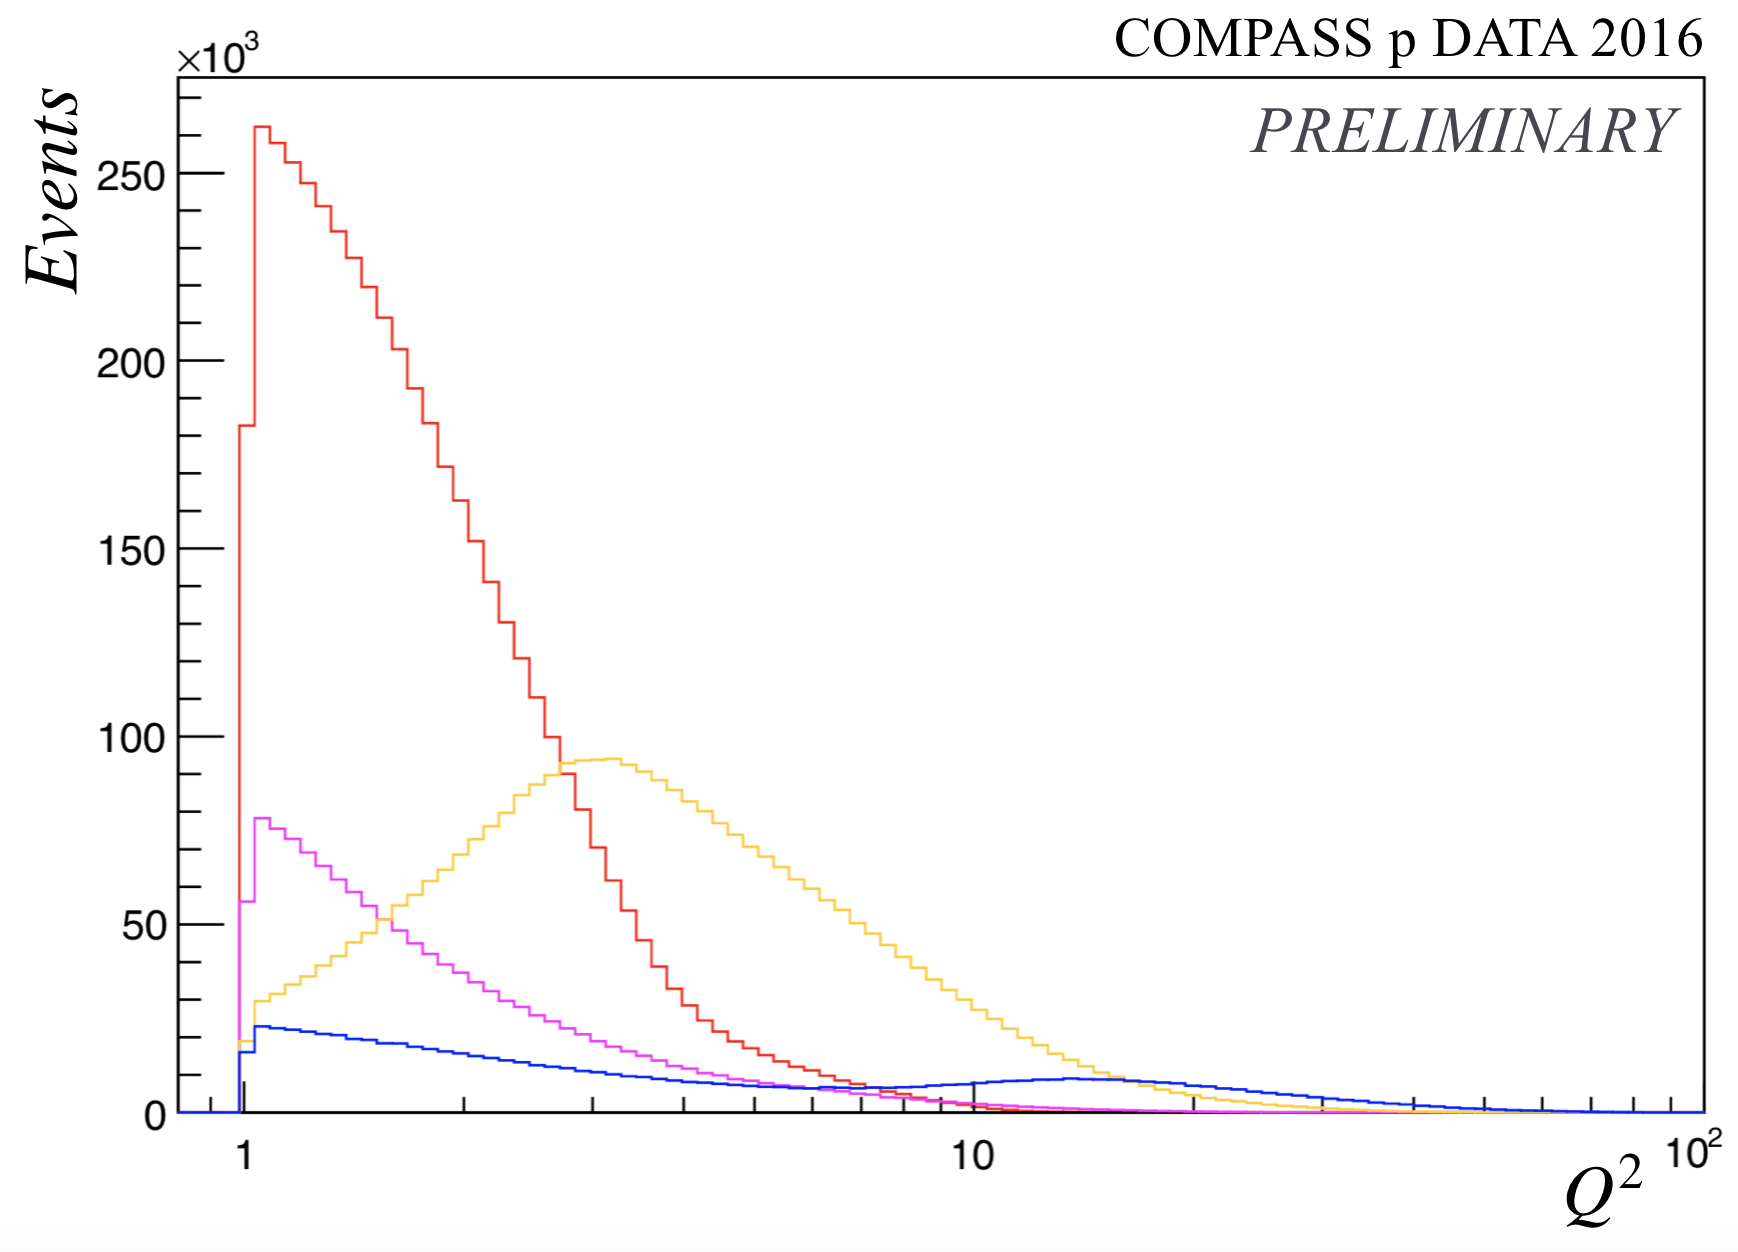
\includegraphics[scale=0.26]{./gfx/Q2trig.png}}
  \subfloat[]{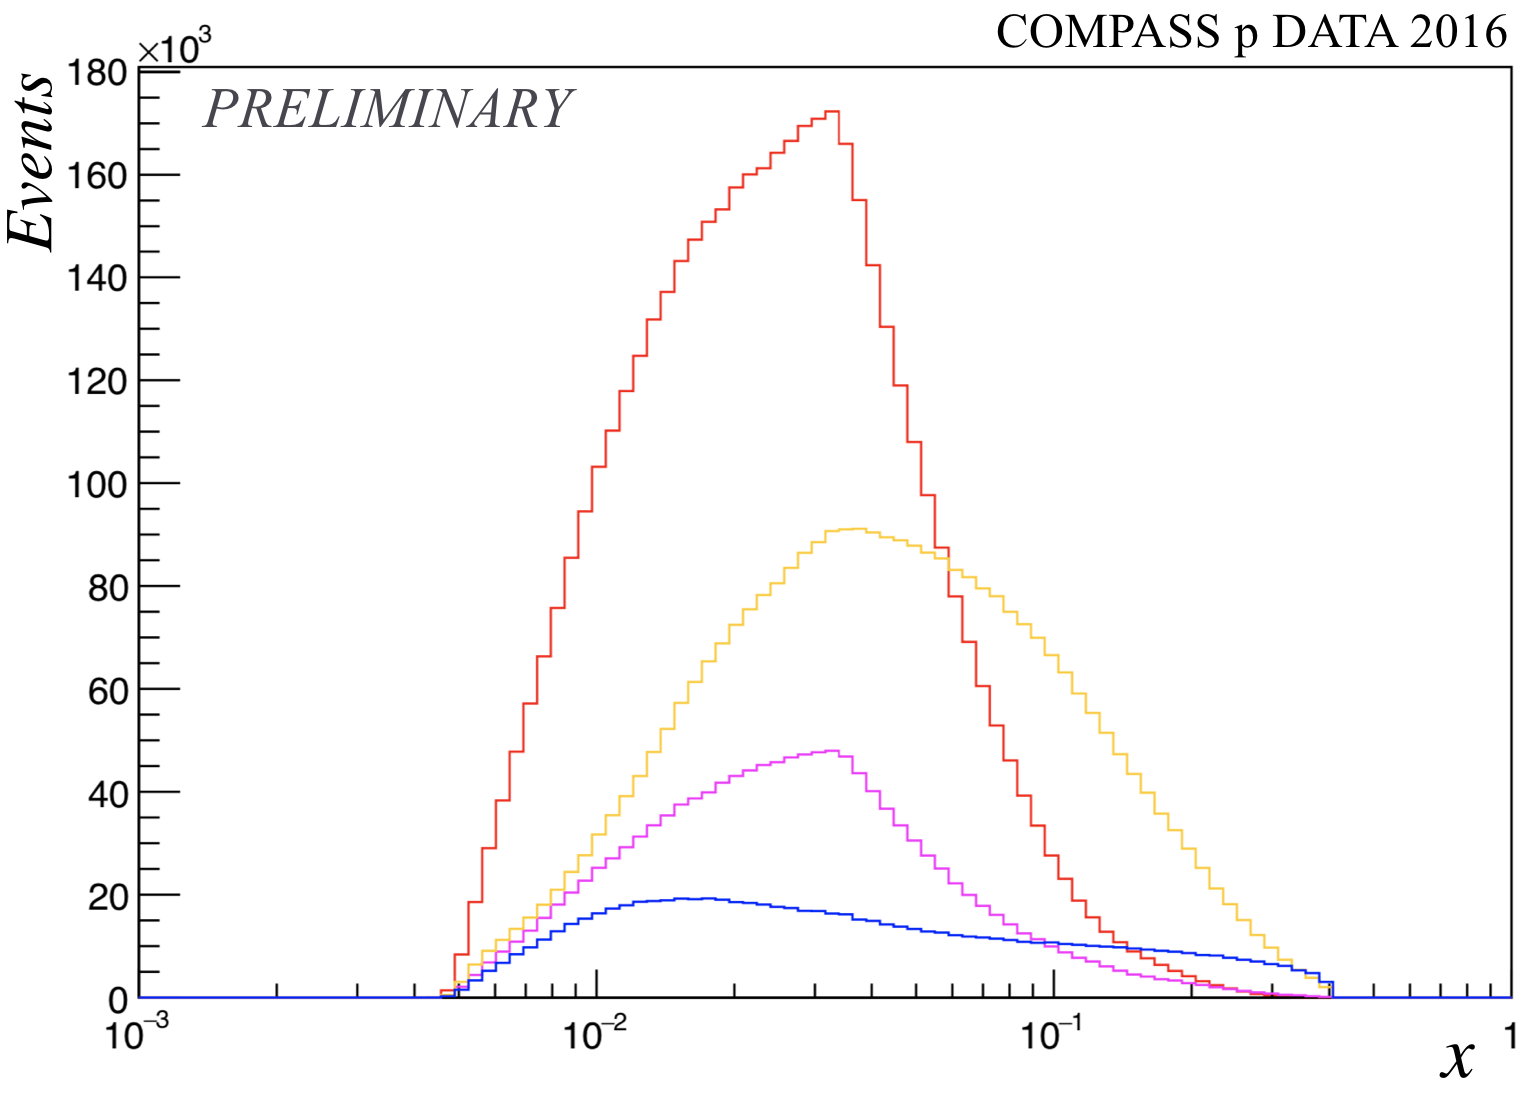
\includegraphics[scale=0.26]{./gfx/xtrig.png}}
	\caption{Event distribution for the middle, ladder, outer and las triggers as a function of $Q^2$ (a) and $x$ (b).}
	\label{pic:triggerxQ2}
\end{figure}

The $Q^2$, $x$ and $y$ distributions are illustrated in Fig.~\ref{pic:DISdist} for the DIS sample after event selections. The $Q^2$-$x$ correlation is also shown as well as the $x$-$y$ one. It can be noted that most of the statistics is located in the low $Q^2$-$x$ and low $x$-$y$ values and $Q^2$ values reach up to 90 (GeV/$c$)$^2$.

\begin{figure}[!h]
  \subfloat[$Q^2$]{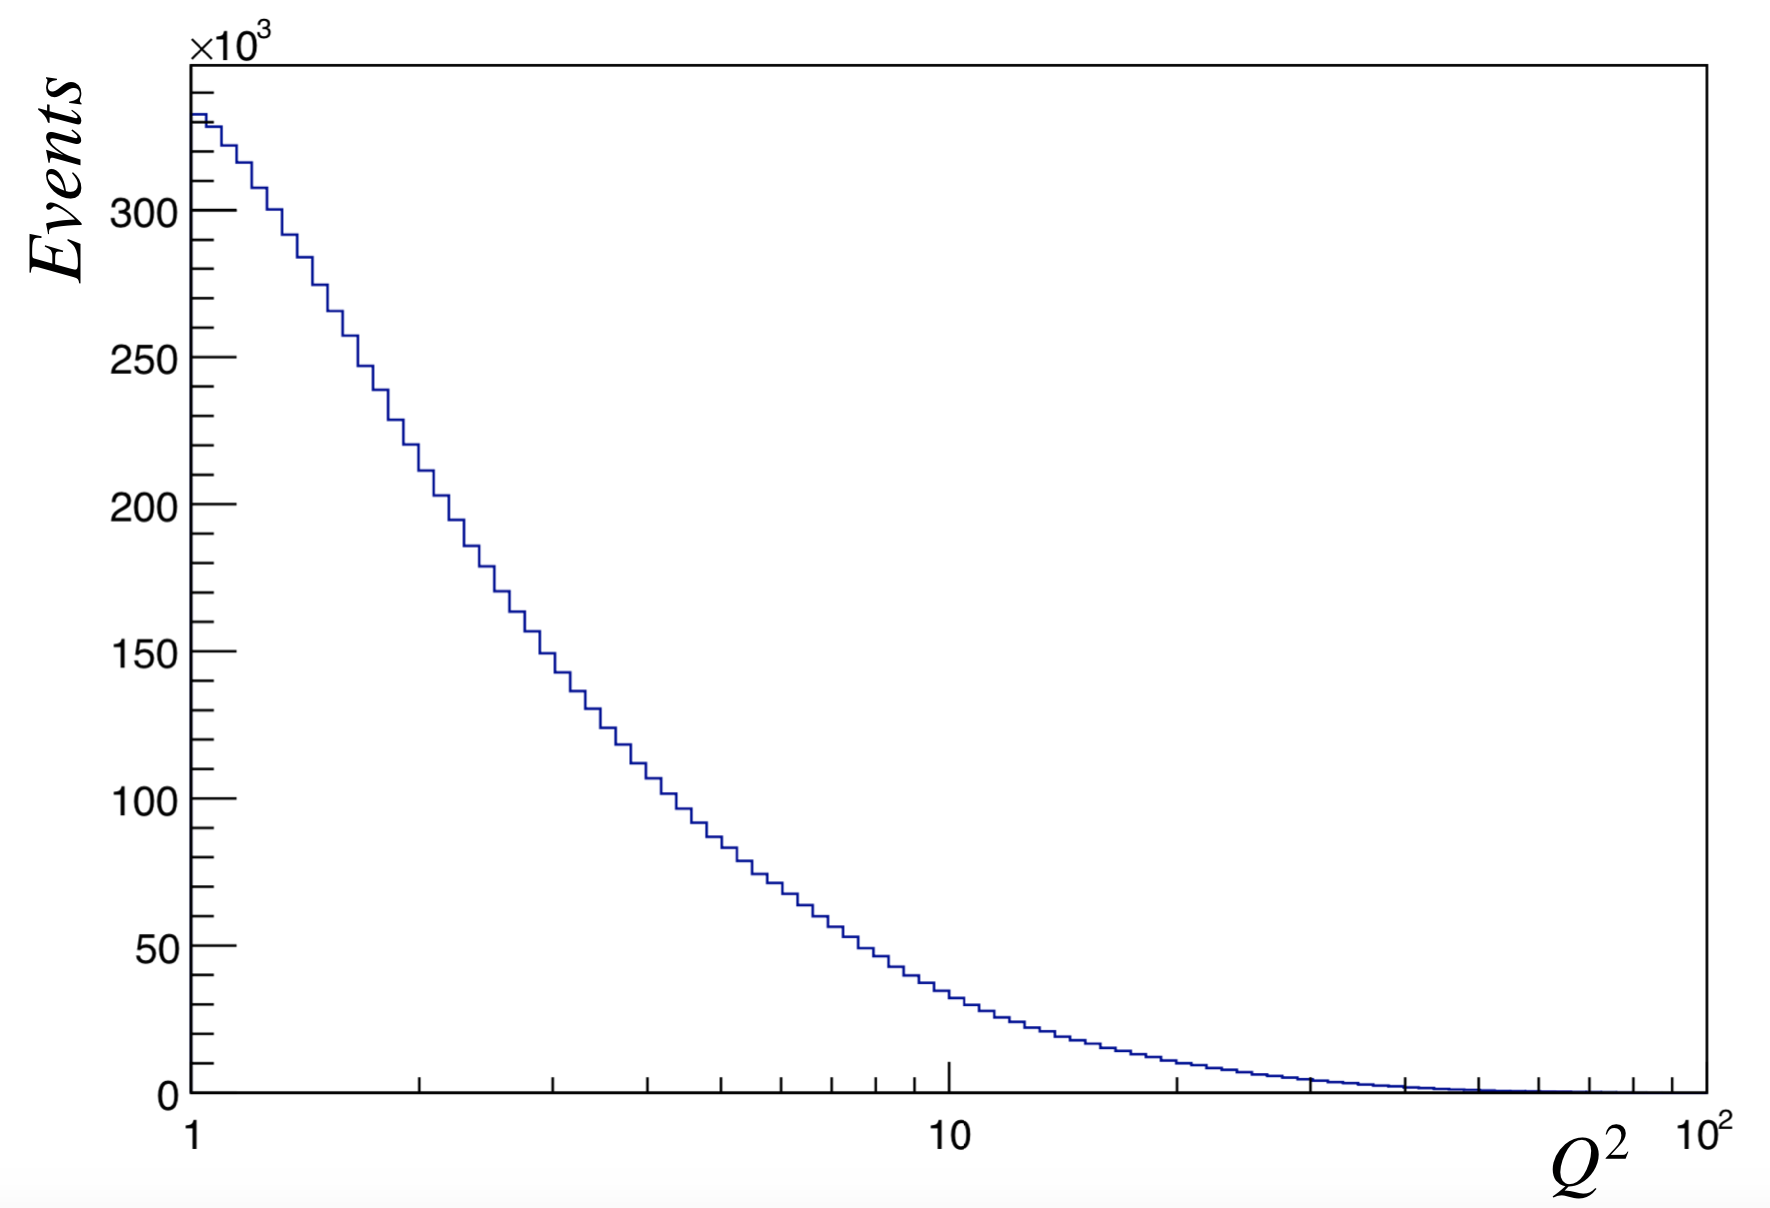
\includegraphics[scale=0.17]{./gfx/Q2DIS.png}}
  \subfloat[$x$]{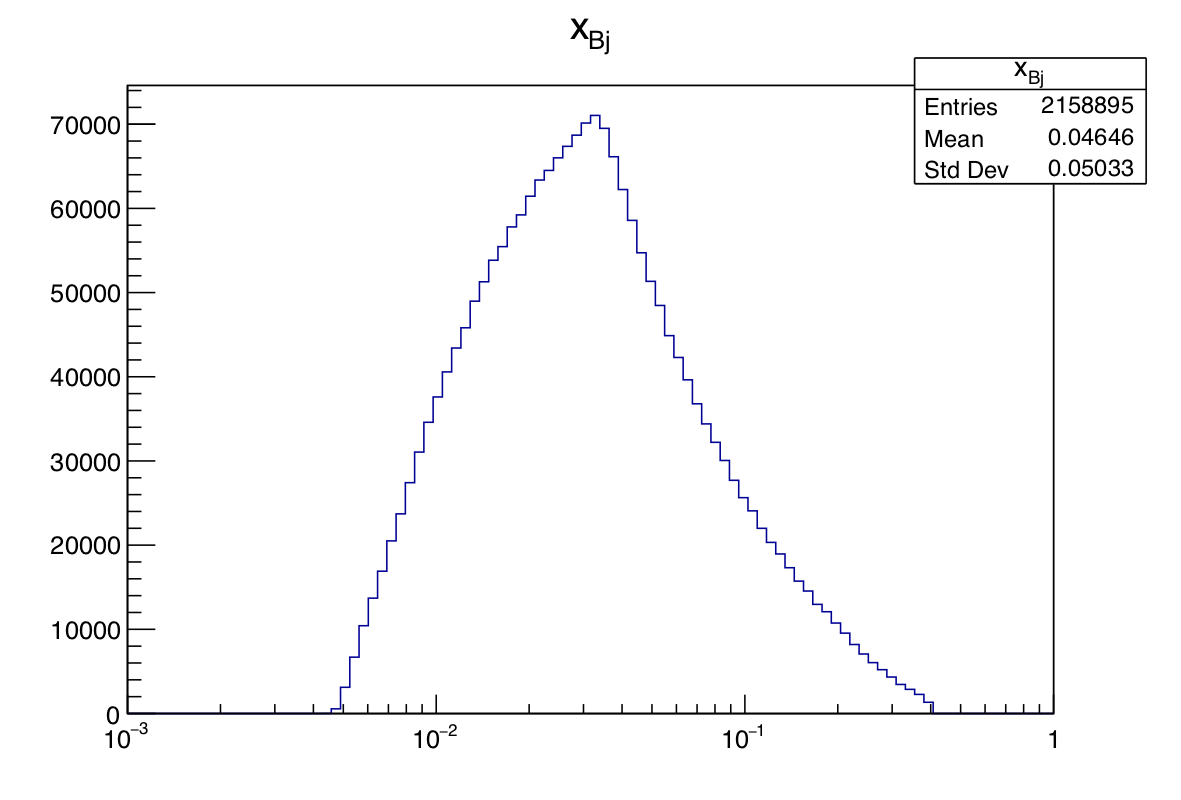
\includegraphics[scale=0.17]{./gfx/xDIS.png}}
  \subfloat[$y$]{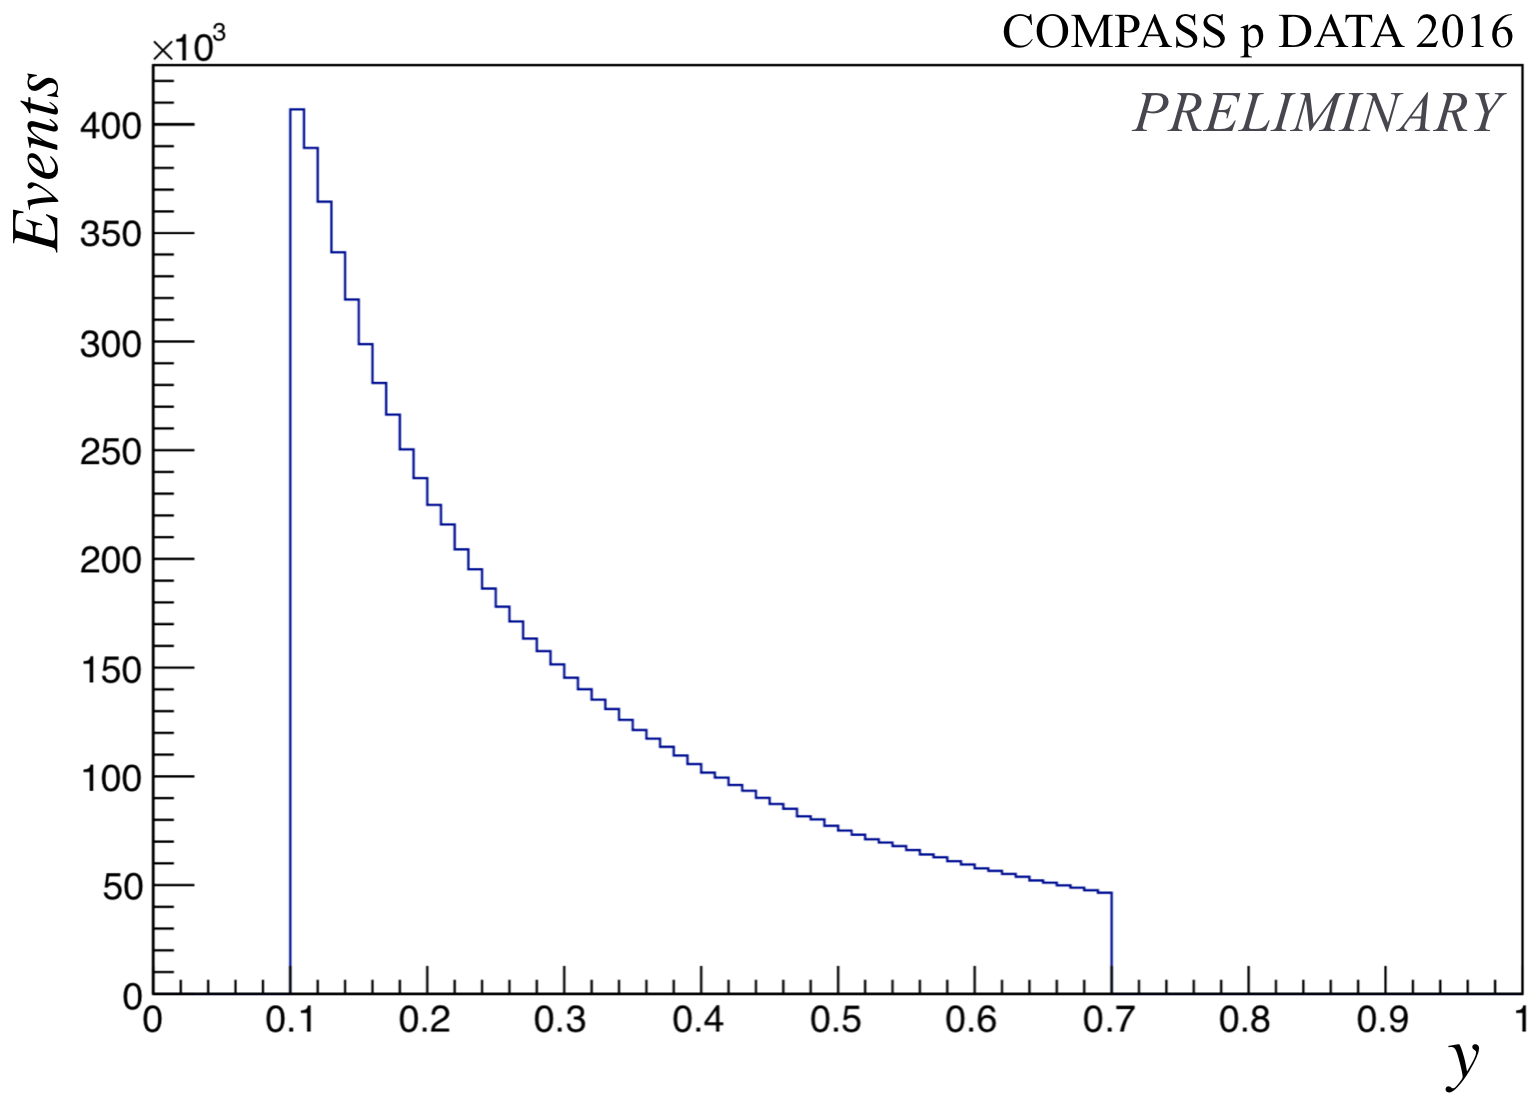
\includegraphics[scale=0.17]{./gfx/yDIS.png}} \\
  \subfloat[$x$-$Q^2$]{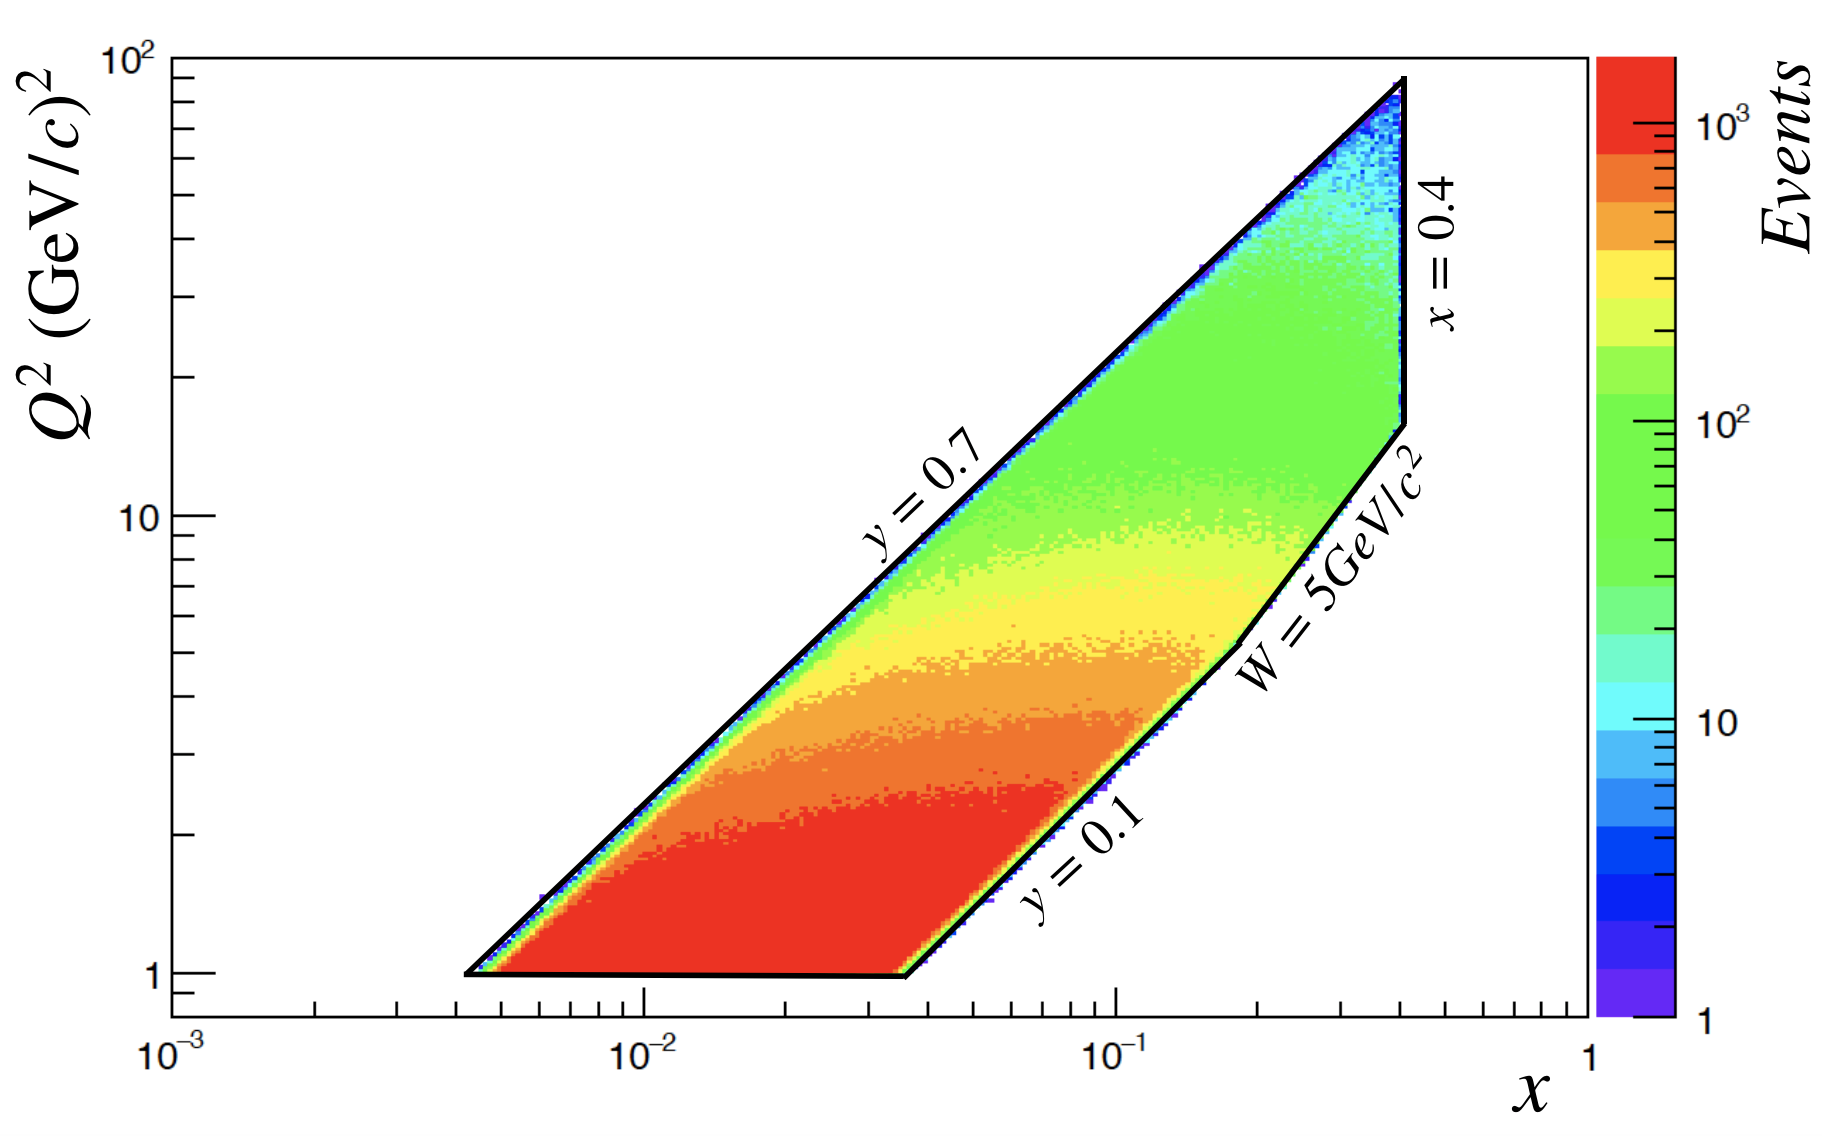
\includegraphics[scale=0.27]{./gfx/xQ2.png}}
  \subfloat[$x$-$y$]{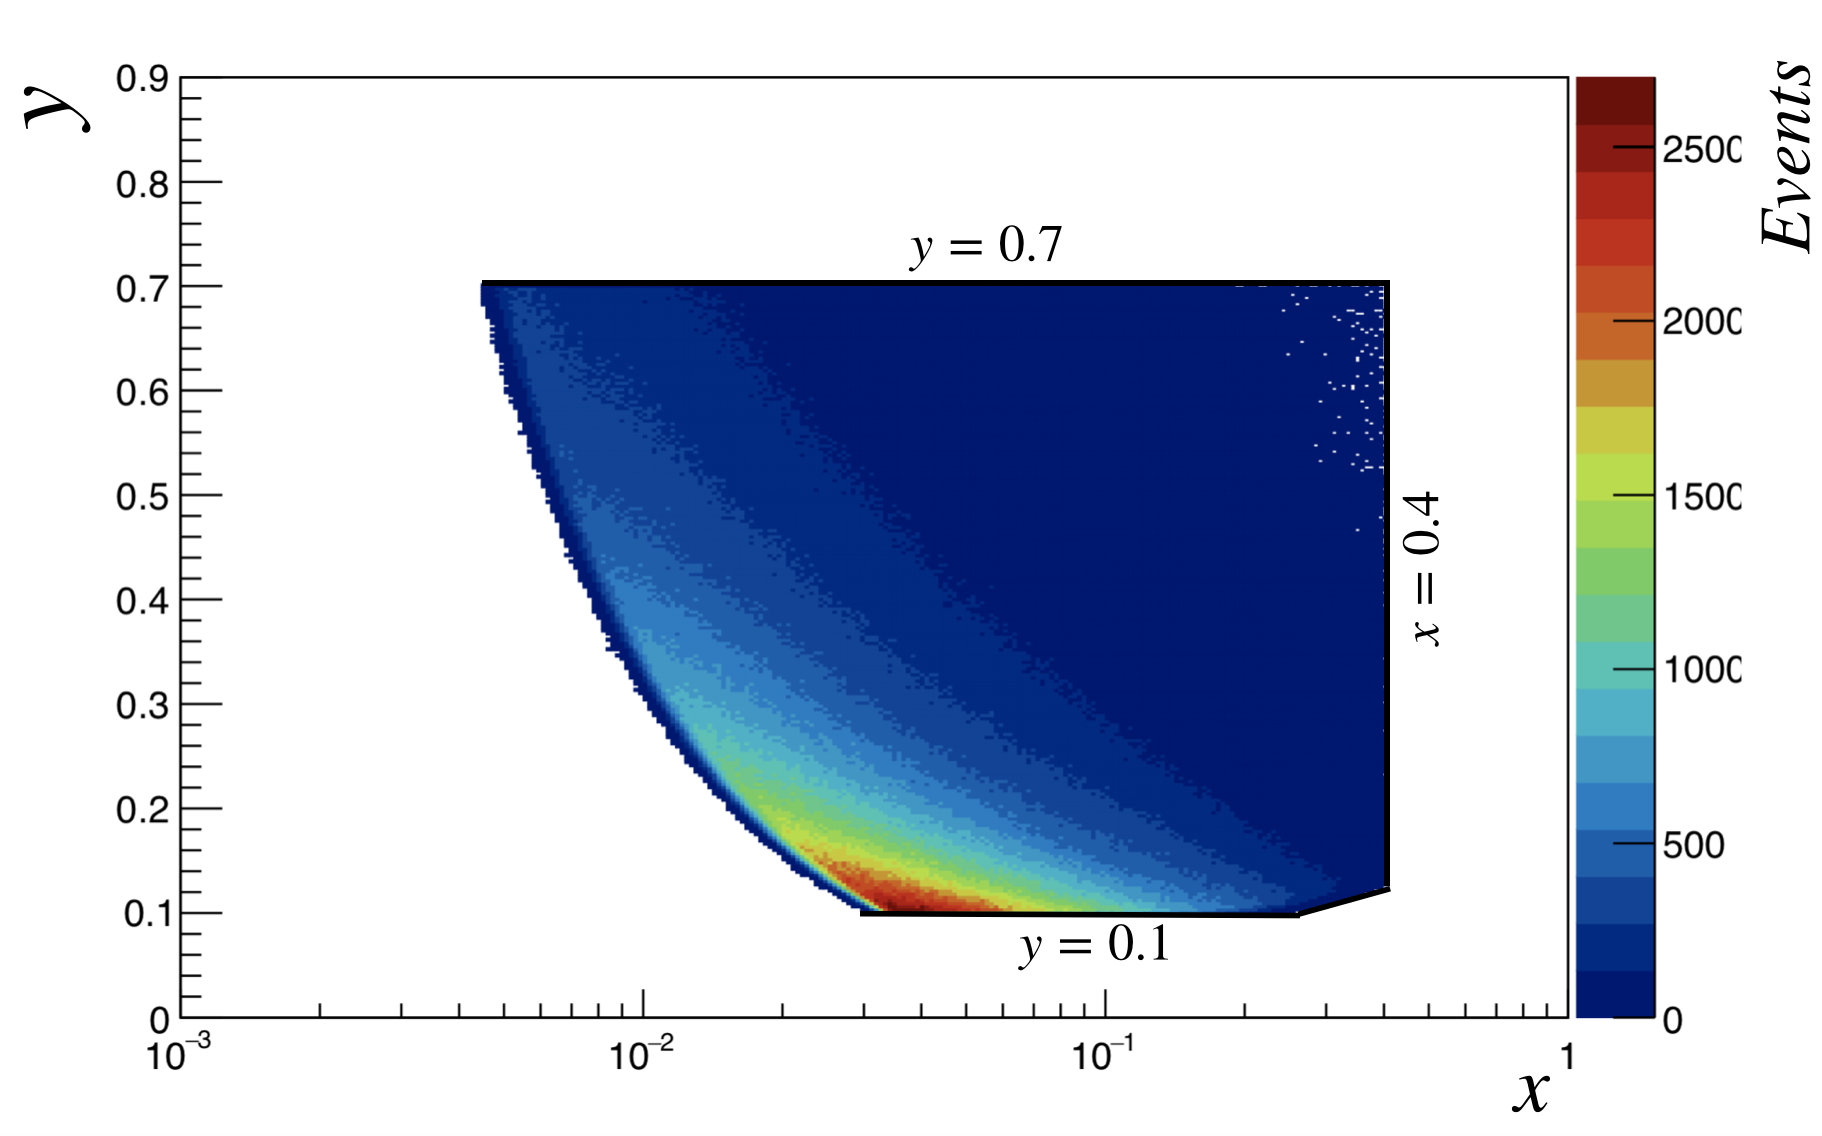
\includegraphics[scale=0.27]{./gfx/xy.png}}
	\caption{On the top panels, $Q^2$, $x$ and $y$ distributions. On the bottom, $x$-$Q^2$ and $x$-$y$ correlations. All distributions are for the final DIS sample.}
	\label{pic:DISdist}
\end{figure}

%------------------------------------------------

\section{Target cut evaluation} \label{sec:targetcut}

The $2.5$ m long $lH_2$ target in $2016$ is not perfectly straight (slight 'banana shaped', Fig.~\ref{pic:Target}) due to the mylar tube. In the Monte-Carlo simulation we use a $2.5$ m long cylinder tilted with respect to the beam by average angles. This angle corresponds to the angle between the upstream and downstream ends of the target. Of course due to its 'banana shape' in reality, the description of the target in Monte-Carlo is not reaching $100$\% fidelity. After the radial cut on the real data target ($1.9$ cm radius) to get rid of the mylar and a cut along $y$ ($y$ = $1.2$ cm) to get rid of the bubbles in the upstream part of the target due to its tilt, the volume of the real data target remaining after intersection with the Monte-Carlo target is of $0.5$\% (Fig.~\ref{pic:Target}). This brings a systematic error on the multiplicities that we wanted to avoid. To this end, we devised three different solutions :

\begin{figure}[!h]
	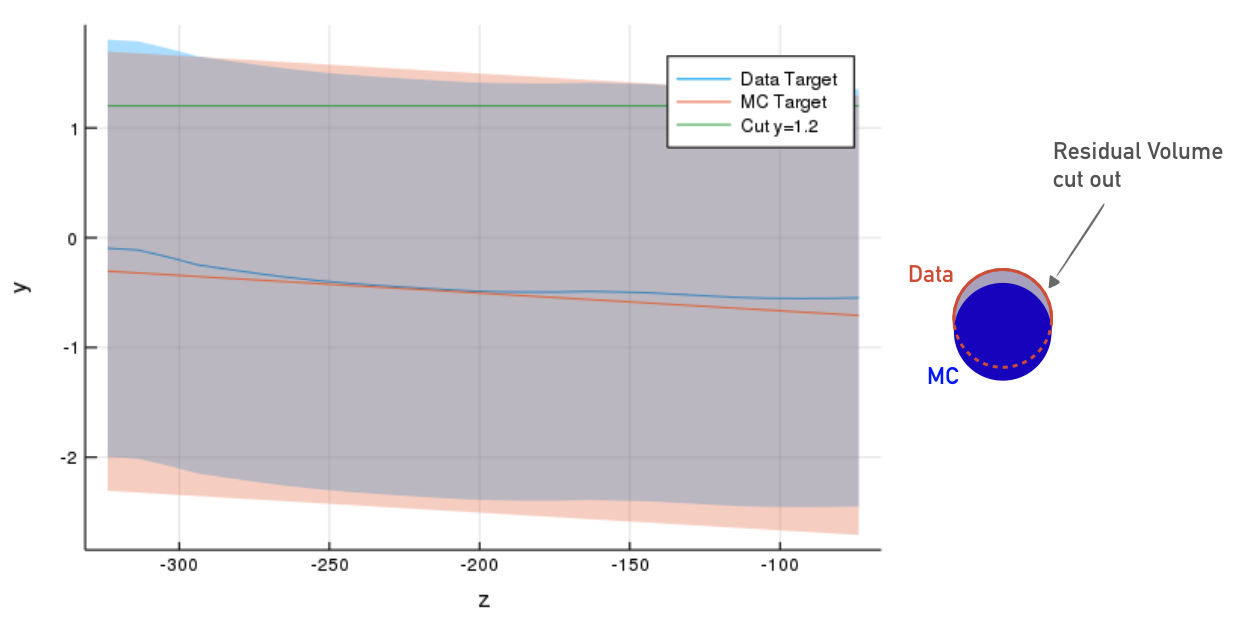
\includegraphics[scale=0.4]{./gfx/Targetcut.png}
	\caption{Left is a ($y$,$z$) view of the real data (blue) and the Monte-Carlo target (red), $z$ being the direction of propagation of the beam. The actual cut used in the analysis corresponds to the intersection of both real data target (red) and Monte-Carlo target (blue) volumes. The green line shows the y = $1.2$ cm cut. Right is a sketch showing the approximate overlap between the two volumes.}
	\label{pic:Target}
\end{figure}

\begin{enumerate}
  \item Cut more severely on the radius of the real data target ($1.7$ cm radial cut) to reduce the non-overlapping volume to zero.
  \item Do a simultaneous cut on the real data target and on the Monte-Carlo target to only keep the overlap between the two volumes.
  \item Do a better description of the target in the Monte-Carlo by using several cylinder volumes and fuse them together to increase the fidelity of the Monte-Carlo target description with respect to the real data one.
\end{enumerate}

The last solution may be used in the future to maximise the efficiency of the analysis from a statistic point of view but it is heavy and time consuming for a marginal gain. This gain is of at most $0.5$\% with respect to the method was eventually chosen, while one can argue that as the events gained are on the edge of the target, thus might be cut out by checking for the muon beam trajectory crossing entirely the target cell, the gain should even be less than this.
The first two solutions were in competition and had the same spirit : cut more in the data target to avoid any systematic bias between real data target and Monte-Carlo target. We chose the second one, a simultaneous cut on both targets, as it was the one that was discarding less target volume, thus maximising statistics. Fig.~\ref{pic:Target} displays the volume that survives such cut.

%------------------------------------------------

\section{Hadron selection}

In the Table~\ref{tab:DIScuts}, the effect of the cuts for hadrons is summarized, showing the number of hadrons and the absolute percentage of the sample remaining :

\begin{table}[!h]
  \centering
  \caption{List and effects of the cuts for hadrons. The percentage corresponds to the absolute percentage of the sample remaining.}
  \label{pic:Hadroncuts}
  \begin{tabular}{p{10cm} p{2cm} p{2cm}}
    \hline
    \hline
     Cut & \# of events after cut & Absolute \% of events after cut  \\
    \hline
    \hline
    Particle is not a scattered muon & 37.0 M & 100\% \\
    Maximum radiation length cumulated along all the trajectory < 15 radiation lengths & 28.3 M & 76.6\% \\
    $\chi^2$/ndf $<$ 10 for the hadron track & 27.9 M & 75.4\% \\
    Z coordinate of the first measured hit < 350 cm & 27.9 M & 75.3\% \\
    Z coordinate of the last measured hit > 350 cm & 19.1 M & 51.5\% \\
    $0.01 < \theta_{RICH} < 0.12$ (at RICH entrance) & 12.6 M & 34.1\% \\
    $x^2_{RICH} + y^2_{RICH} > 25$ cm$^2$ (rejection of RICH pipe) & 12.5 M & 33.7\% \\
    $12 < p_h < 40$ GeV/$c$ & 3.37 M & 9.11\% \\
    $0.2 < z < 0.85$ & 2.67 M & 7.21\% \\
    Events in the specified $\nu$ range & - & - \\
    \hline
    \hline
  \end{tabular}
\end{table}

+ explain it was already present in DIS table.
The cut on the kinematic variable $\nu$ was already present in the DIS table as it is a cut that cuts on both DIS events and hadrons. The cut was implemented to reject events that contain hadrons outside of the measured momentum range of $12$ - $40$ GeV/$c$. The criteria is defined by :
%
\begin{equation}
  \nu_{max} = \frac{\sqrt{(p^2_{max}+m^2_h)}}{z_{max}},
\end{equation}
\begin{equation}
  \nu_{min} = \frac{\sqrt{(p^2_{min}+m^2_h)}}{z_{min}},
\end{equation}
%
where $p_{max}$ ($p_{min}$) is the hadron momentum limit of $40$ GeV/$c$ ($12$ GeV/c), $z_{max}$ ($z_{min}$) is the upper (lower) value of the $z$-bin and $m_h$ is the mass of the considered hadron. As the cut depends on the mass of the considered hadron, the number of DIS events is different for each identified hadron.

%------------------------------------------------

\section{Downstream target vertex distribution}

We discovered when looking at vertex distribution for hadrons and comparing data with Monte-Carlo that there was a deficit of about $6$\% of vertices at the downstream part of the target (between -$100$ and -$70$ cm as shown in Fig.~\ref{VertexDrop}). This phenomenon is observed both in data and Monte-Carlo however it was more pronounced in data than in Monte-Carlo. After investigation, I discovered that, both in data and Monte-Carlo, there were hadrons that have their track not attached to the best primary vertex in a $2$ mm-radius circle around the best primary vertex (Fig.~\ref{CircleHadron}). This contribution is only found in the downstream part of the target while in the upstream part it is non-existant.

\begin{figure}[!h]
	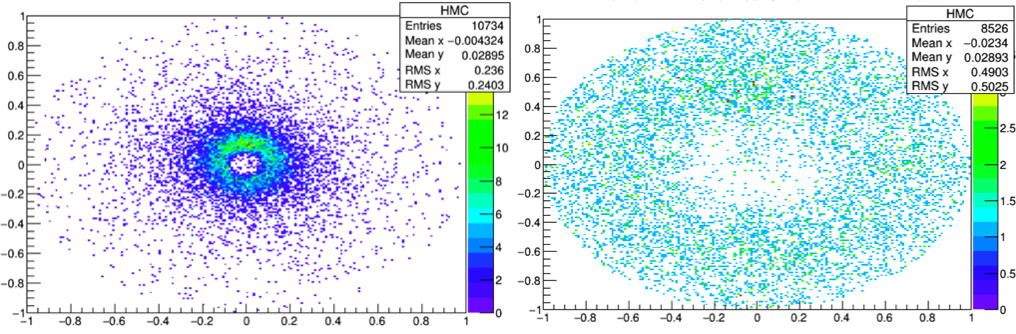
\includegraphics[scale=0.45]{./gfx/CircleHadron.png}
	\caption{The relative distance to the best primary vertex of the extrapolated position of the unattached hadrons to the vertex position perpendicular to the beam direction. On the left, the plot corresponds to the downstream part of the target and on the right, to the upstream part.}
	\label{CircleHadron}
\end{figure}

This problem is introduced by the reconstruction software and could not be solved in time for this thesis. However we found a rescue procedure to reattach these hadrons to the best primary vertex. All the hadrons in a circle of radius $2$ mm around the best primary vertex are used in the further analysis as if they were attached to it. The same quality cuts were applied to these hadrons as for the attached ones. With this procedure we were able to recover for the loss of hadron in the downstream part of the target as seen in Fig.~\ref{VertexDrop}.

\begin{figure}[!h]
	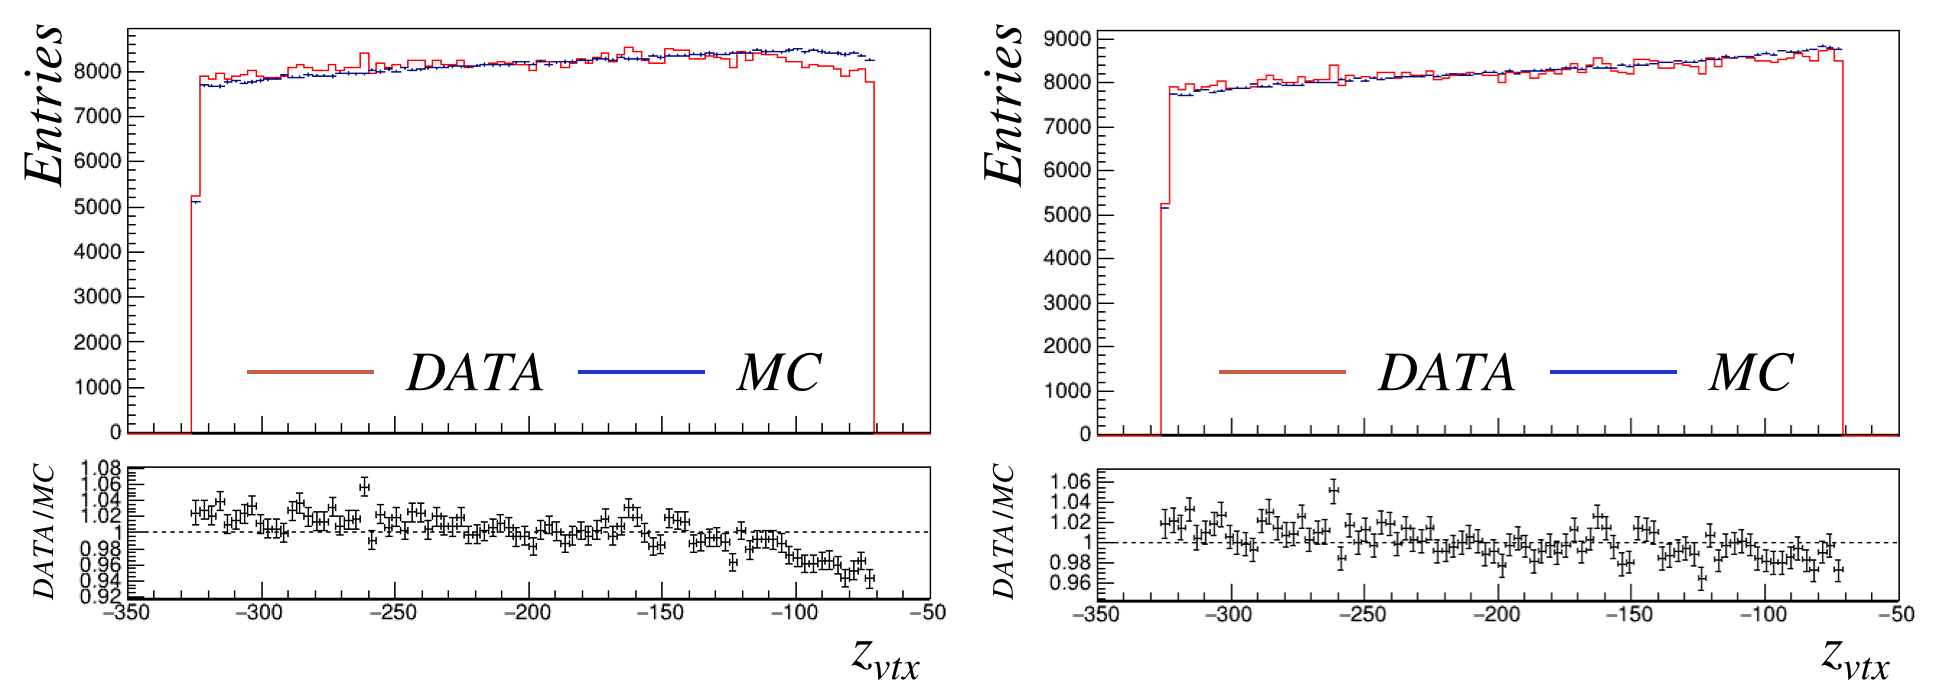
\includegraphics[scale=0.45]{./gfx/VertexDrop.png}
	\caption{Comparison of the vertex distribution along the target of data and MC hadrons left) before and right) after the rescue procedure.}
	\label{VertexDrop}
\end{figure}

%----------------------------------------------------------------------------------------

\section{Particle Identification with RICH detector}

The $\pi$ and $K$ particle identification (PID) is performed by the RICH detector.

The method used for the RICH particle identification is described in Chapter. \ref{ch:PID}. The idea is the following : when a particle is detected, six likelihood (LH) functions are calculated ($\pi$, $K$, $p$, $e$, $\mu$ and the background) and are then compared to make the particle identification. The evaluation is done separately for pions, kaons and protons. The largest value corresponds to the maximal probability. The method is improved by looking further to $LH(2^{nd})$, which is the second highest value of the four compared likelihood values ($\pi$, $K$, $p$ and the background). The electron and muon likelihoods are not considered in the assignment of $LH(2^{nd})$ as in the chosen momentum range (12 to 40 GeV/c) the RICH detector can not be used to efficiently distinguish electrons from $\pi$.

All $\pi$, $K$ and $p$ probabilities are needed for the unfolding. The likelihood cuts were optimized as in Table~\ref{tab:LHcut} of Chapter~\ref{ch:PID} with some additional conditions as this is not a clean sample :

\begin{enumerate}
  \item Pion selection
  \begin{itemize}
    \item $LH(\pi) > 0$
    \item $LH(\pi) > LH(K)$, $LH(p)$ and $LH(bg)$.
  \end{itemize}
  \item Kaon selection
  \begin{itemize}
    \item $LH(K) > 0$
    \item $LH(K) > LH(\pi)$, $LH(p)$ and $LH(bg)$.
  \end{itemize}
  \item Proton selection
  Three cases are considered depending on the momentum $p_{h}$ of the particle and are distinguished by the kaon threshold ($\simeq 8.9$ GeV/c) and proton threshold ($\simeq 17.95$ GeV/c) :
  \begin{enumerate}[(a)]
    \item Kaon threshold $< p_{h} \leq$ proton threshold - 5 GeV/c
    \begin{itemize}
      \item All LH = $0$
    \end{itemize}
    \item $p_{h} >$ proton threshold + 5 GeV/c
    \begin{itemize}
      \item $LH(p) > 0$
      \item $LH(p) > LH(\pi)$, $LH(K)$ and $LH(bg)$.
    \end{itemize}
    \item Proton threshold - 5 GeV/c $< p_{h} <$ proton threshold + 5 GeV/c
    \begin{itemize}
      \item Using (a) and (b) simultaneously.
    \end{itemize}
  \end{enumerate}
\end{enumerate}

%----------------------------------------------------------------------------------------

\section{RICH unfolding based on efficiency matrices}

With the unfolding procedure the hadron identification is corrected on a hadron by hadron basis for the limited RICH efficiency and misidentification.
In order to perform this correction, the RICH actual performance was evaluated from real data in Chapter~\ref{ch:PID}. The result of
this evaluation is presented through RICH performance matrices, $M_{RICH}$, binned in momentum
and angle :

\begin{itemize}
  \item $p_h$ \{12,13,15,17,19,22,25,27,30,35,40\} GeV/c
  \item $\theta$ \{0.01,0.04,0.12\} rad
\end{itemize}

The $3$-by-$3$ matrices $M_{RICH}$ give a relation between the vector of counts for true hadron $T_h$ and the vector for identified hadron $I_h$ :
%
\begin{equation}
\begin{bmatrix}
I_{\pi} \\
I_K \\
I_p
\end{bmatrix}
=
\begin{bmatrix}
\epsilon(\pi \rightarrow \pi) & \epsilon(K \rightarrow \pi) & \epsilon(p \rightarrow \pi)\\
\epsilon(\pi \rightarrow K) & \epsilon(K \rightarrow K) & \epsilon(p \rightarrow K) \\
\epsilon(\pi \rightarrow p) & \epsilon(K \rightarrow p) & \epsilon(p \rightarrow p)
\end{bmatrix}
\begin{bmatrix}
T_{\pi} \\
T_K \\
T_p
\end{bmatrix}.
\end{equation}
%
The coefficients of the $M_{RICH}$, $\epsilon(t \rightarrow i)$, are the probabilities that a true hadron of type
$t$ is identified as a hadron of type $i$.

The number of true hadrons are obtained by inverting the performance matrices (Eq.~\ref{richmat}) :
%
\begin{equation}
  \overrightarrow{T_h} = M^{-1}_{RICH}\overrightarrow{I_h}.
	\label{richmat}
\end{equation}
%
\begin{table}[!h]
  \caption{\label{HadNum} Number of identified pions, kaons, and protons for the five analyzed periods before and after unfolding.}
  \centering
  \begin{tabular}{lcccccc}
    \hline
     & $\pi^+$ & $\pi^-$ & $K^+$ & $K^-$ & $p$ & $\bar{p}$ \\
    \hline
    Identified & 953970 & 789480 & 253045 & 153440 & 131066 & 60705 \\
    Unfolded & 976213 & 814685 & 255132 & 150775 & 124221 & 52014 \\
    \hline
  \end{tabular}
\end{table}

%----------------------------------------------------------------------------------------

\section{Kinematic binning}

The multiplicities are evaluated in bins of the Bjorken variable $x$, the muon energy fraction carried by the virtual photon $y$ and the virtual photon energy fraction carried by final state hadron $z$. They are calculated with the following formula :
%
\begin{equation}
  \frac{dM^h(x,y,z)}{dz}=\frac{1}{N^{DIS}_{Events}(x,y)}\frac{dN^{DIS}_{h}(x,y,z)}{dz},
\end{equation}
%
where $N^{DIS}_{Events}$ is the number of DIS events and $N^{DIS}_{h}$ is the number of
hadrons after RICH unfolding. As in practise, the multiplicities are measured in bins of
x (9 bins), y (5 bins) and z (12 bins), the raw multiplicities (multiplicities without corrections) can be expressed as :
%
\begin{equation}
  M^h_{raw}(x,y,z) = \frac{N^{DIS}_{h}(x,y,z)/\delta z}{N^{DIS}_{Events}(x,y)},
\end{equation}
%
where $\delta z$ is the width of the z bin. For the multiplicities extraction, the binning in
$x$, $y$ and $z$ is the following :

\begin{table}[!h]
  \centering
  \caption{Multidimensional binning for the multiplicity extraction}
  \label{tab:kinbinning}
  \begin{tabular}{ll}
    \hline
    \hline
    Variable & Binning \\
    \hline
    \hline
    $x$ & \{$0.004,0.01,0.02,0.03,0.04,0.06,0.1,0.14,0.18,0.4$\} \\
    $y$ & \{$0.1,0.15,0.2,0.3,0.5,0.7$\} \\
    $z$ & \{$0.2,0.25,0.3,0.35,0.4,0.45,0.5,0.55,0.6,0.65,0.7,0.75,0.85$\} \\
    \hline
    \hline
  \end{tabular}
\end{table}

%----------------------------------------------------------------------------------------

\section{Statistical error propagation}

The statistical error propagation used in the multiplicity calculation will be explained in the following. All further calculations are done in bins of ($x$,$y$,$z$). All the DIS events enter with the same weight of $1$ in the error calculation :
%
\begin{equation}
		E^2_{DIS} = N_{DIS}.
\end{equation}
%
Same for unidentified hadrons :
%
\begin{equation}
		E^2_{Had} = N_{Had}.
\end{equation}
%
For identified hadrons, the squared error includes the RICH statistical error :
%
\begin{equation}
		E^2_{Had} = \sum_{i=1}^{N_{Had}} E^2_{RICH,i},
\end{equation}
%
where
%
\begin{equation}
		E^2_{RICH}[0<h<3] = cov(M^{-1}_{hr},M^{-1}_{hr})+(M^{-1}_{hr})^2,
\end{equation}
%
with $M_{hr}$ the element of the RICH unfolding matrix for hadron $h$ from RICH identified hadron $r$ and
%
\begin{equation}
		cov(M^{-1}_{hr},M^{-1}_{hr}) = \sum_{0<i,j,k,l<3} M^{-1}_{hi}M^{-1}_{jr}M^{-1}_{hk}M^{-1}_{lr}cov(M_{ij},M_{kl}).
\end{equation}
%
For the raw multiplicities the error takes into account the correlation between hadrons and DIS events :
%
\begin{equation}
		E^2_{raw} = \Bigg[\frac{E^2_{Had}}{N^2_{DIS}} - \bigg( \frac{N^2_{Had}}{N^2_{DIS}} \bigg)^2 E^2_{DIS} \Bigg]/z^2_{width}.
\end{equation}
%
\section{Results for raw multiplicities ($h^{\pm}$, $\pi^{\pm}$, $K^{\pm}$ and $p/\bar{p}$)}

The raw multiplicity results shown in this section are without any correction except the RICH unfolding correction for identified hadrons. The unidentified hadron multiplicities are displayed as a function of $z$ in bins of $x$ and staggered vertically with $y$ in Figs.~\ref{pic:rawhp} to \ref{pic:rawhm} (see Appendix~\ref{app:mult} for identified hadrons). The charged hadron multiplicities strongly depends on $z$ as expected with a small dependence with $x$ also.

The $h^+$/$h^-$, $\pi^+$/$\pi^-$ and $p/\bar{p}$ raw multiplicities are very similar but with a small asymmetry at high $x$, explained by the fact that at high $x$ in the valence region, the $u$ quark is dominant in the target. For kaons, $M_{raw}^{K^+} > M_{raw}^{K^-}$ as $K^-$ ($\bar{u}s$) can be produced by sea quarks or subleading particles.

In total each charged hadron multiplicities yield more than $300$ data points.

\begin{figure}[!h]
	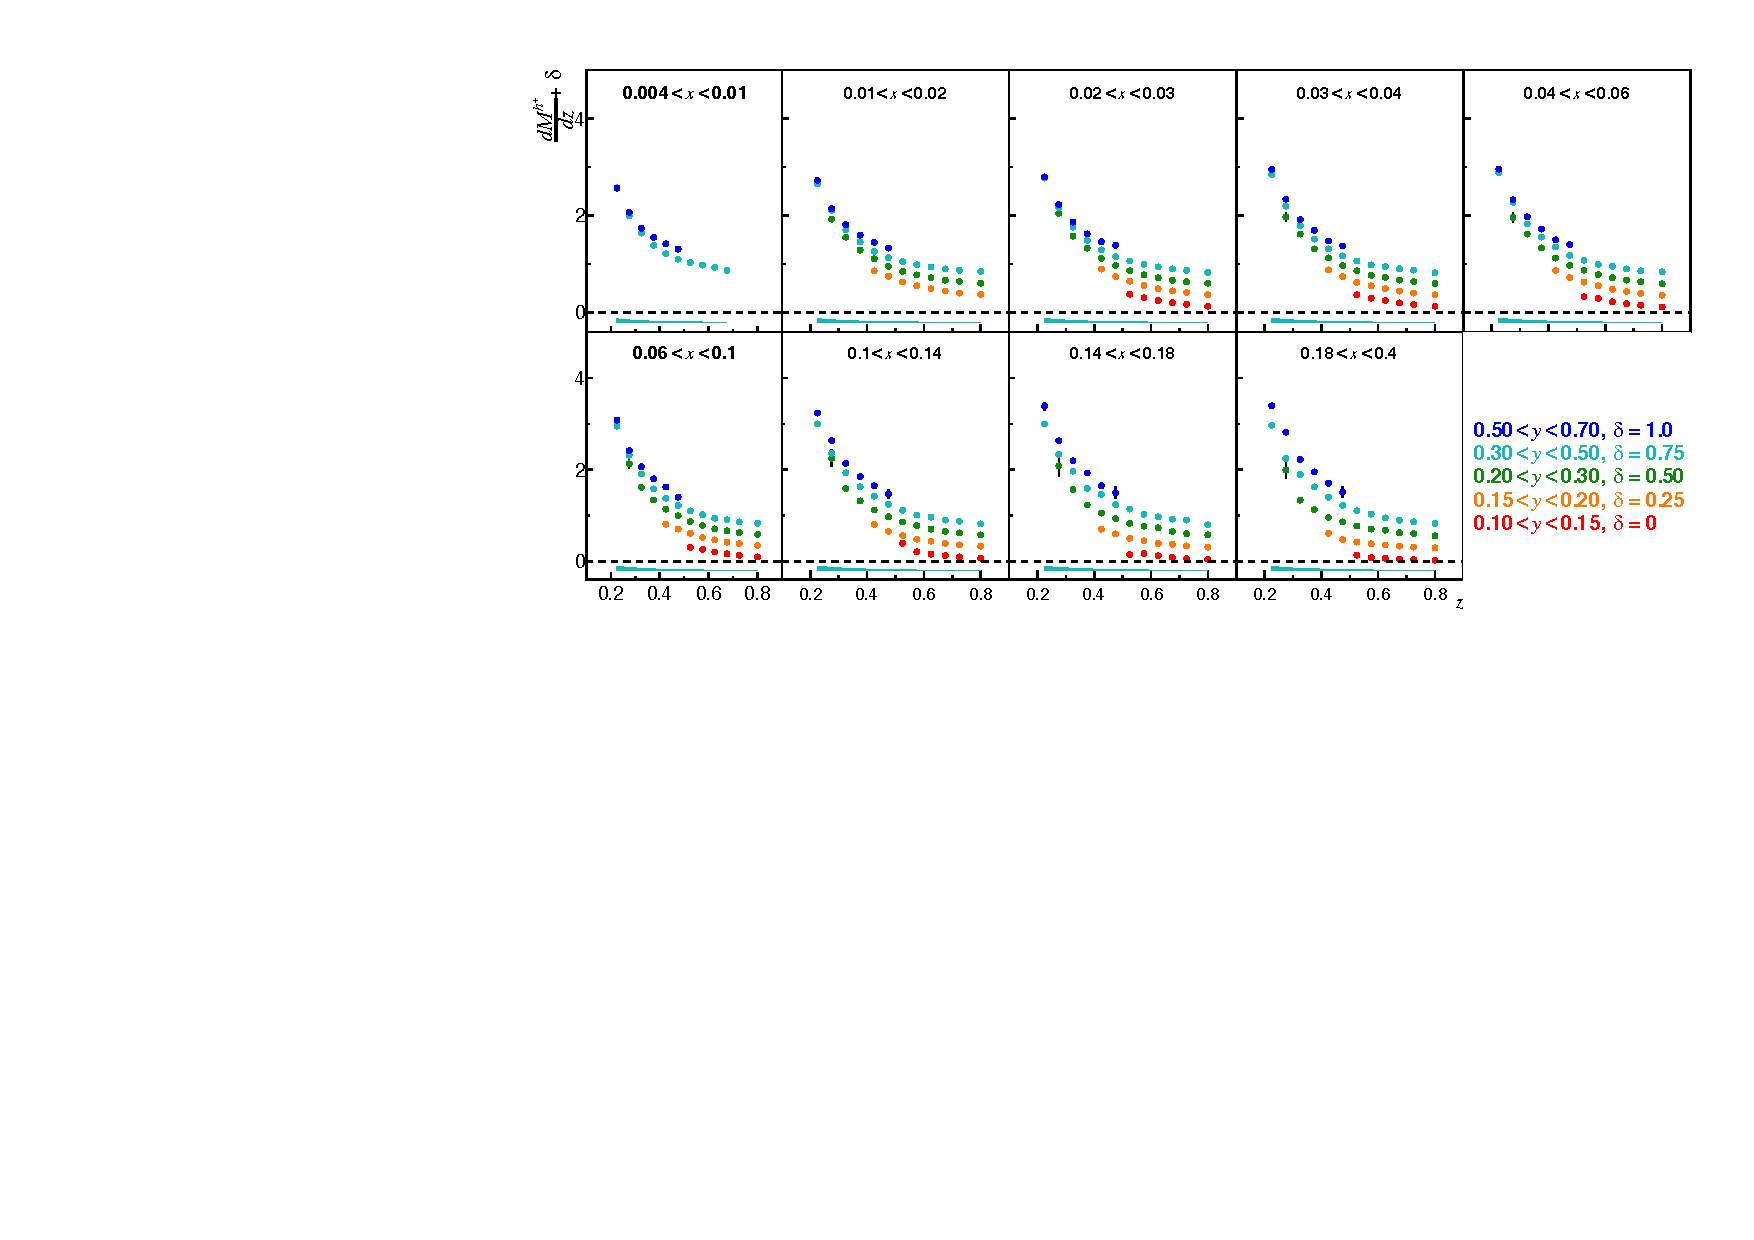
\includegraphics[scale=0.85]{./gfx/rawhp.pdf}
	\caption{Unidentified positive hadron raw multiplicities as a function of $z$ in bins of $x$ and scattered vertically with $y$. Statistical error is shown but is small in most of the bins.}
	\label{pic:rawhp}
\end{figure}

\newpage

\begin{figure}[!h]
  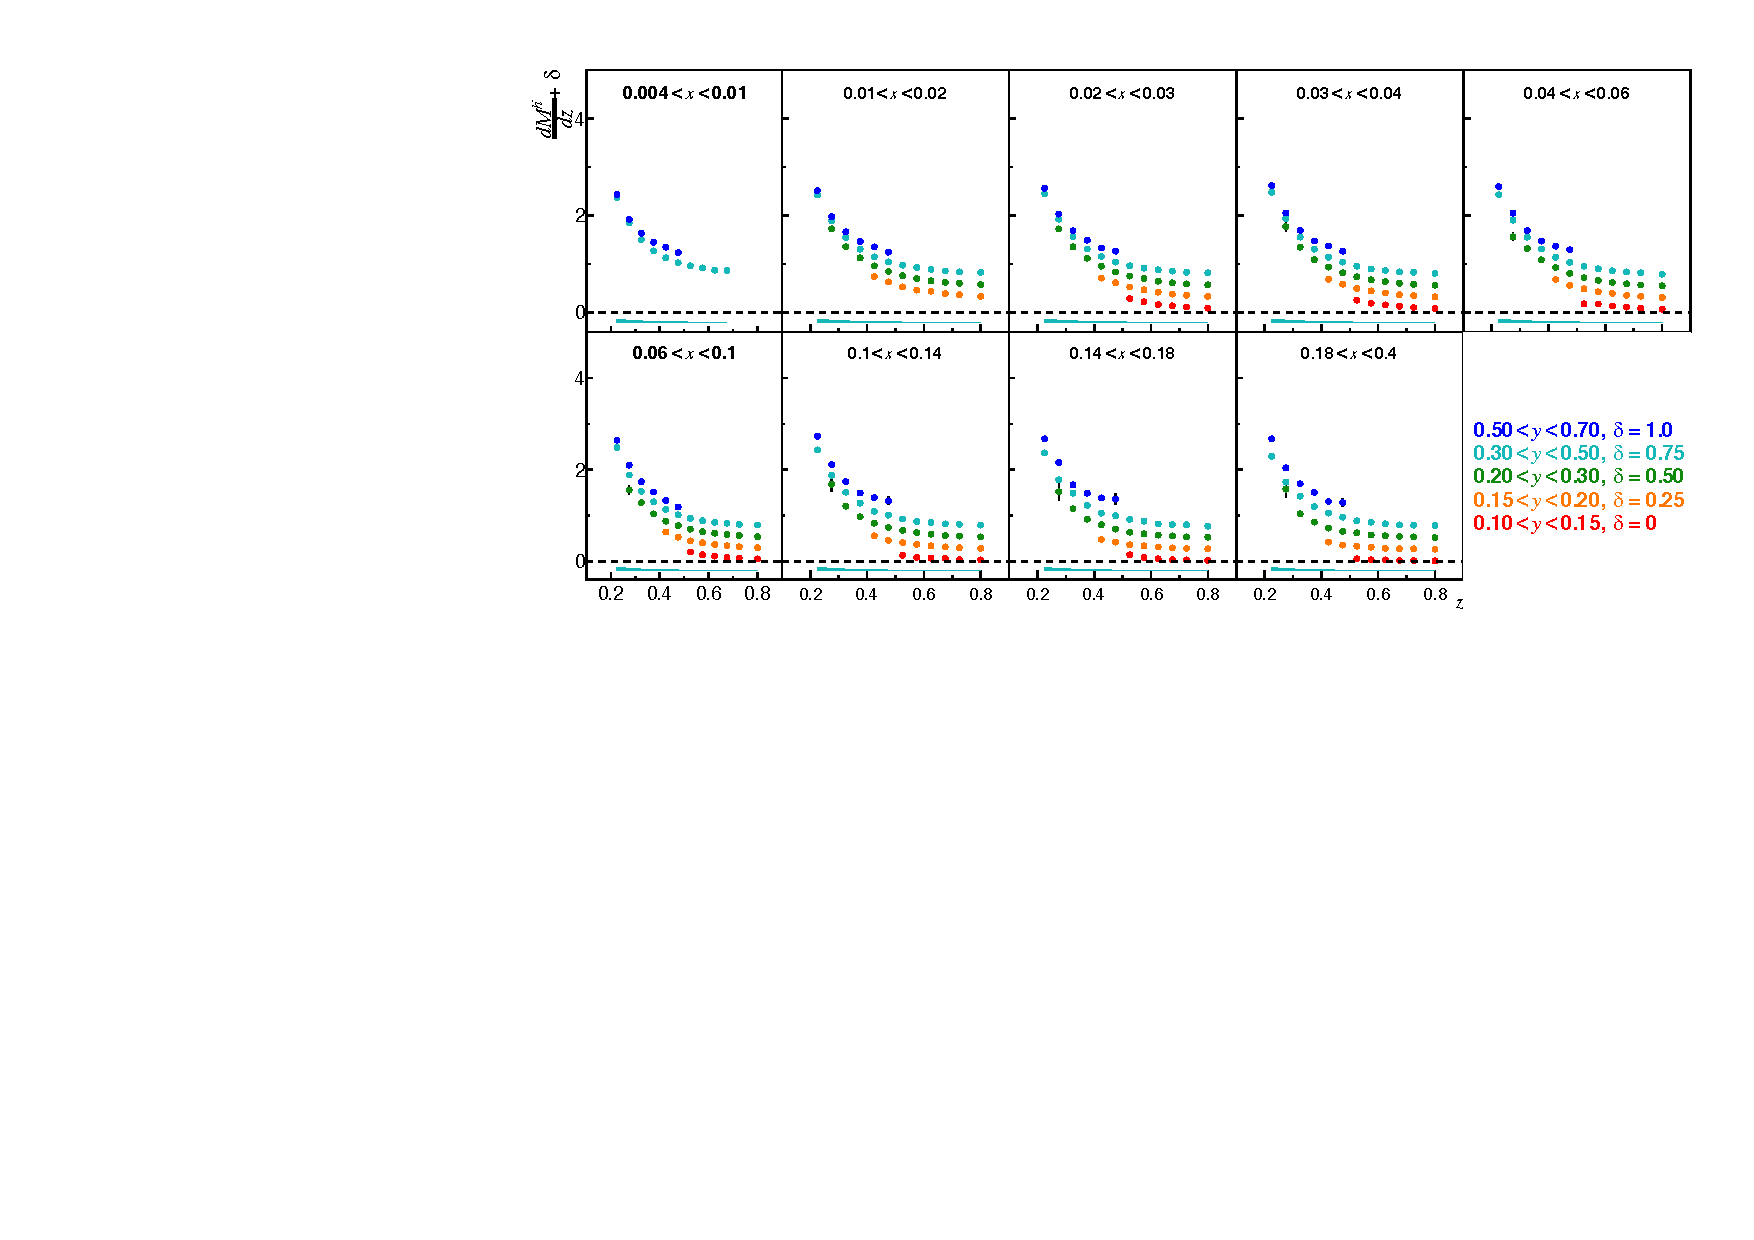
\includegraphics[scale=0.85]{./gfx/rawhm.pdf}
  \caption{Same as Fig.~\ref{pic:rawhp} but for unidentified negative hadrons.}
  \label{pic:rawhm}
\end{figure}

\begin{figure}[!h]
  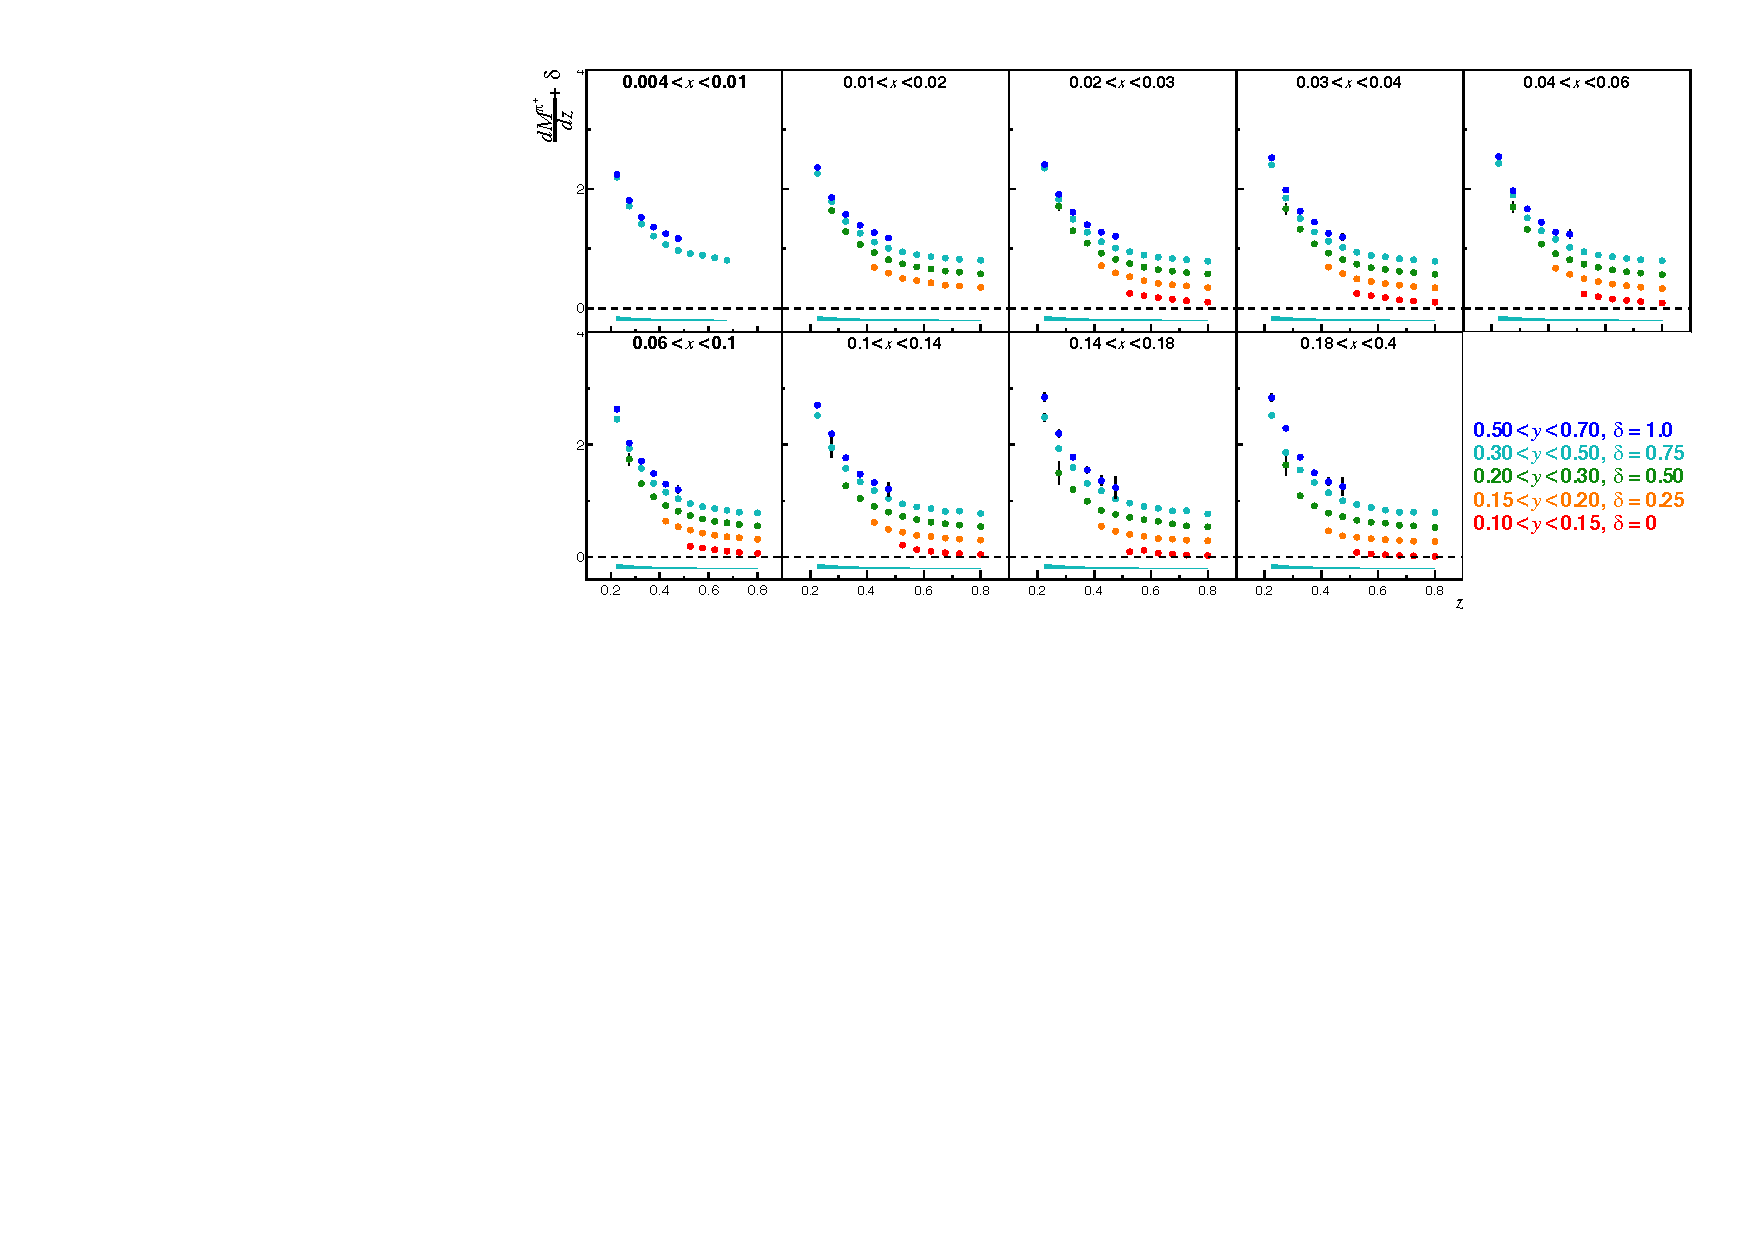
\includegraphics[scale=0.85]{./gfx/rawpip.pdf}
  \caption{Same as Fig.~\ref{pic:rawhp} but for positive pions.}
  \label{pic:rawpip}
\end{figure}

\newpage

\begin{figure}[!h]
  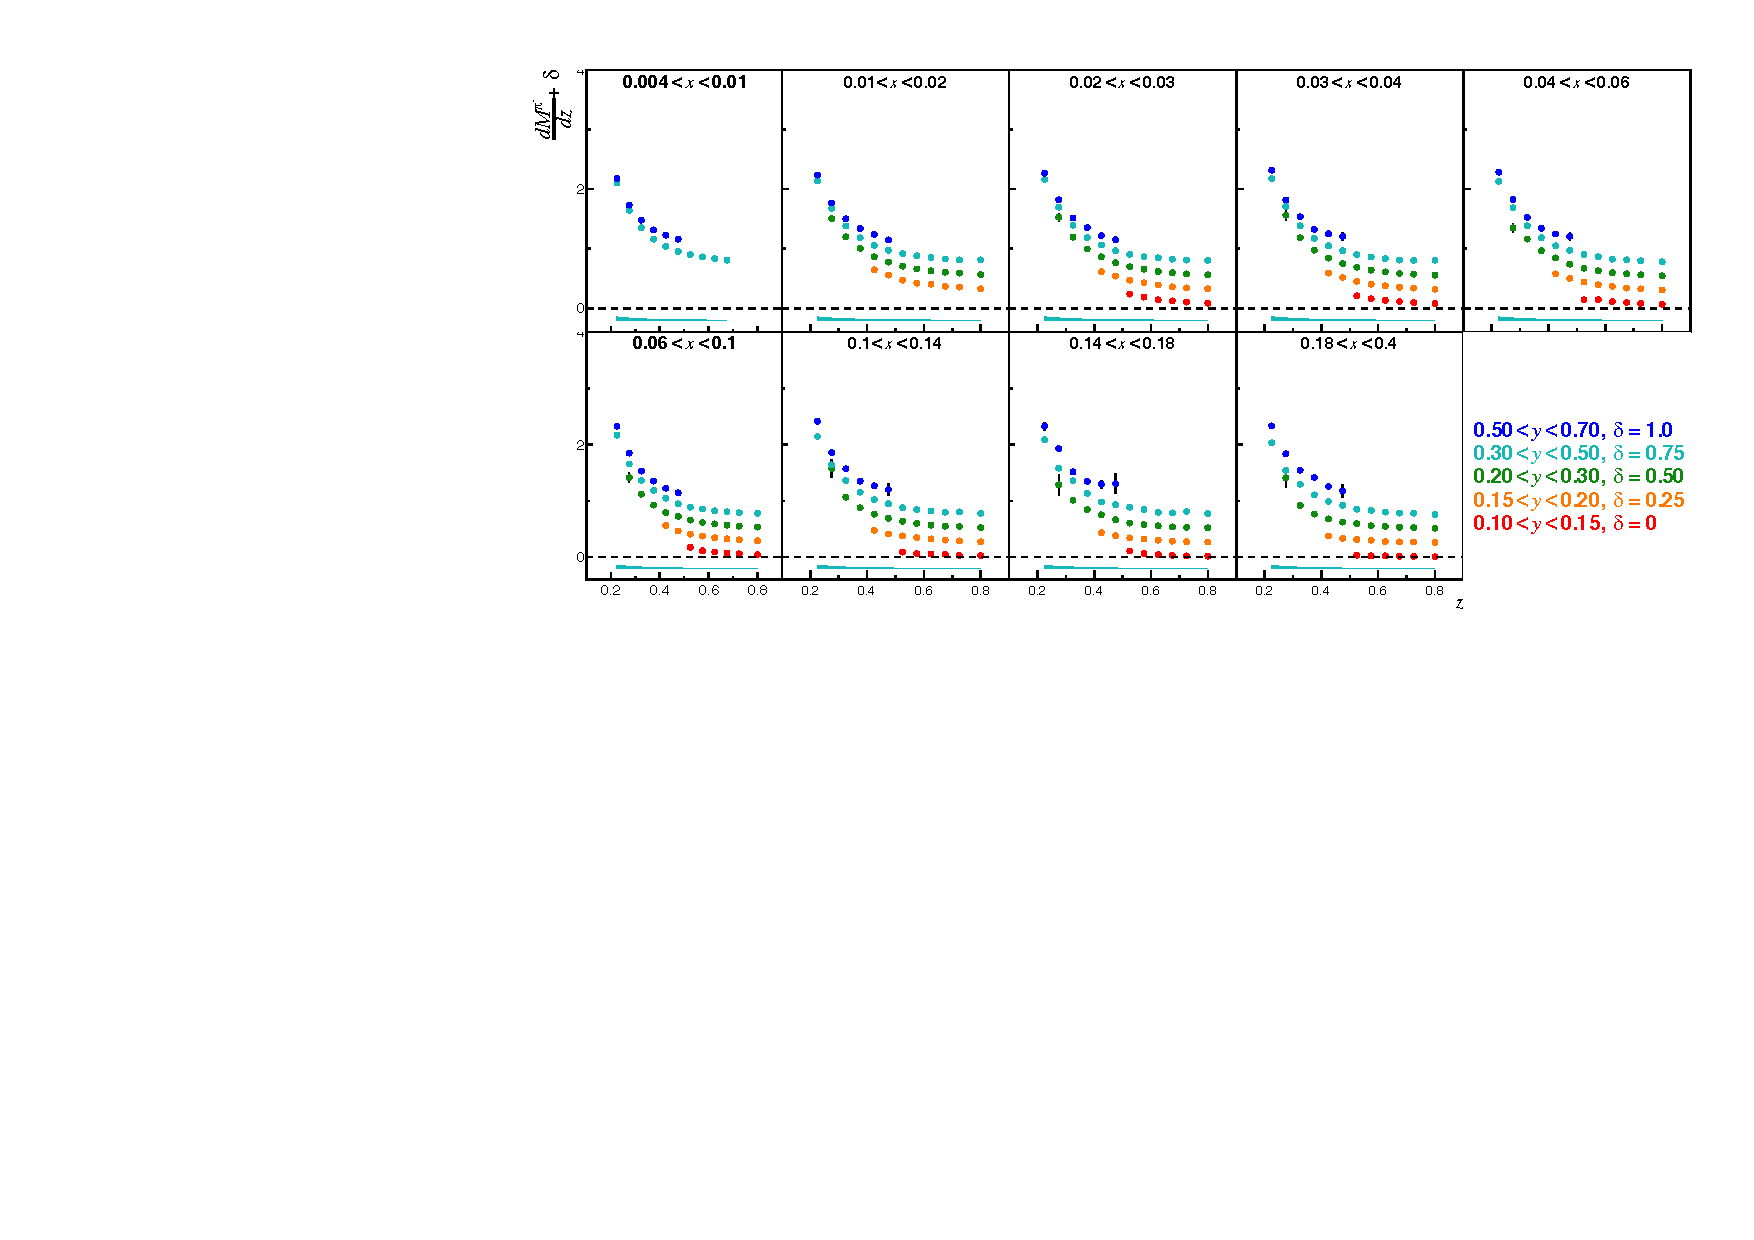
\includegraphics[scale=0.85]{./gfx/rawpim.pdf}
  \caption{Same as Fig.~\ref{pic:rawhp} but for negative pions.}
  \label{pic:rawpim}
\end{figure}

\begin{figure}[!h]
  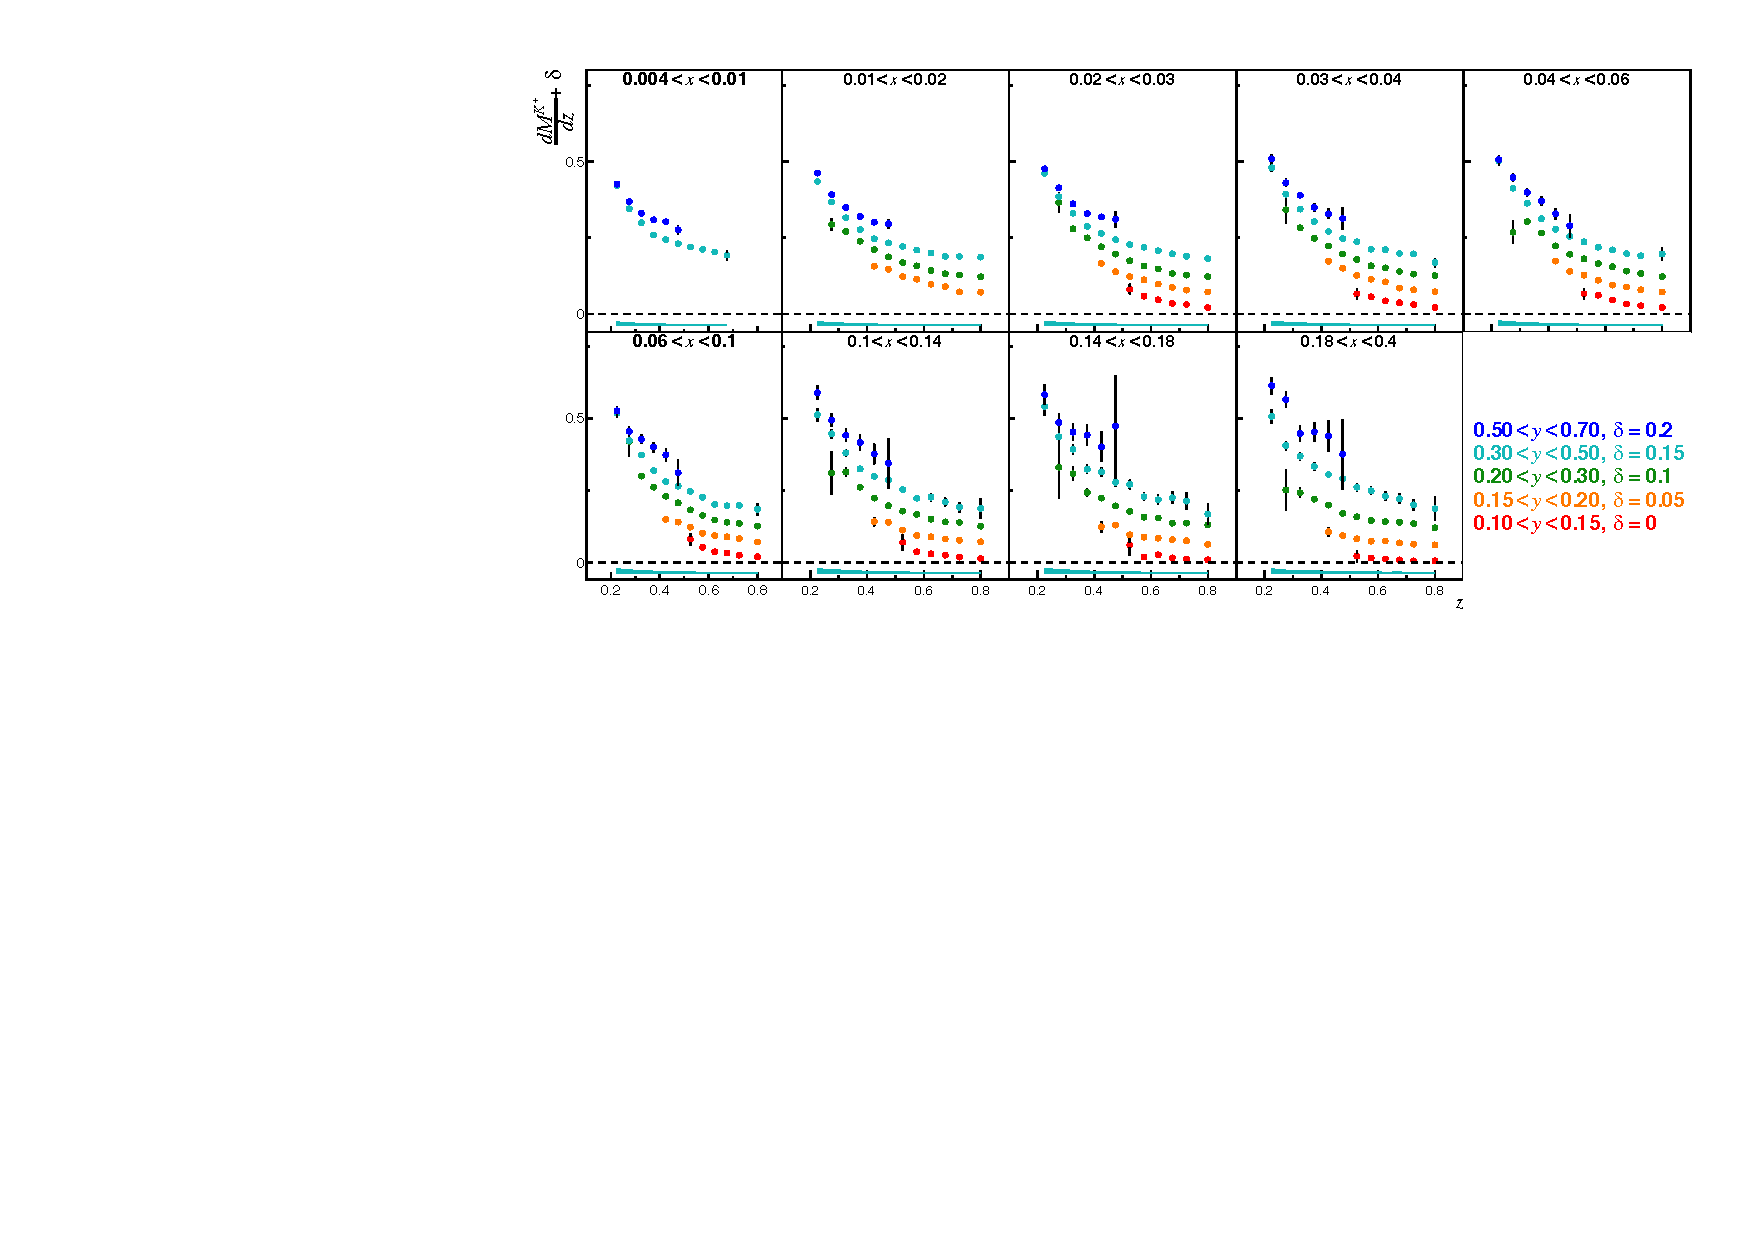
\includegraphics[scale=0.85]{./gfx/rawkp.pdf}
  \caption{Same as Fig.~\ref{pic:rawhp} but for positive kaons.}
  \label{pic:rawkp}
\end{figure}

\newpage

\begin{figure}[!h]
  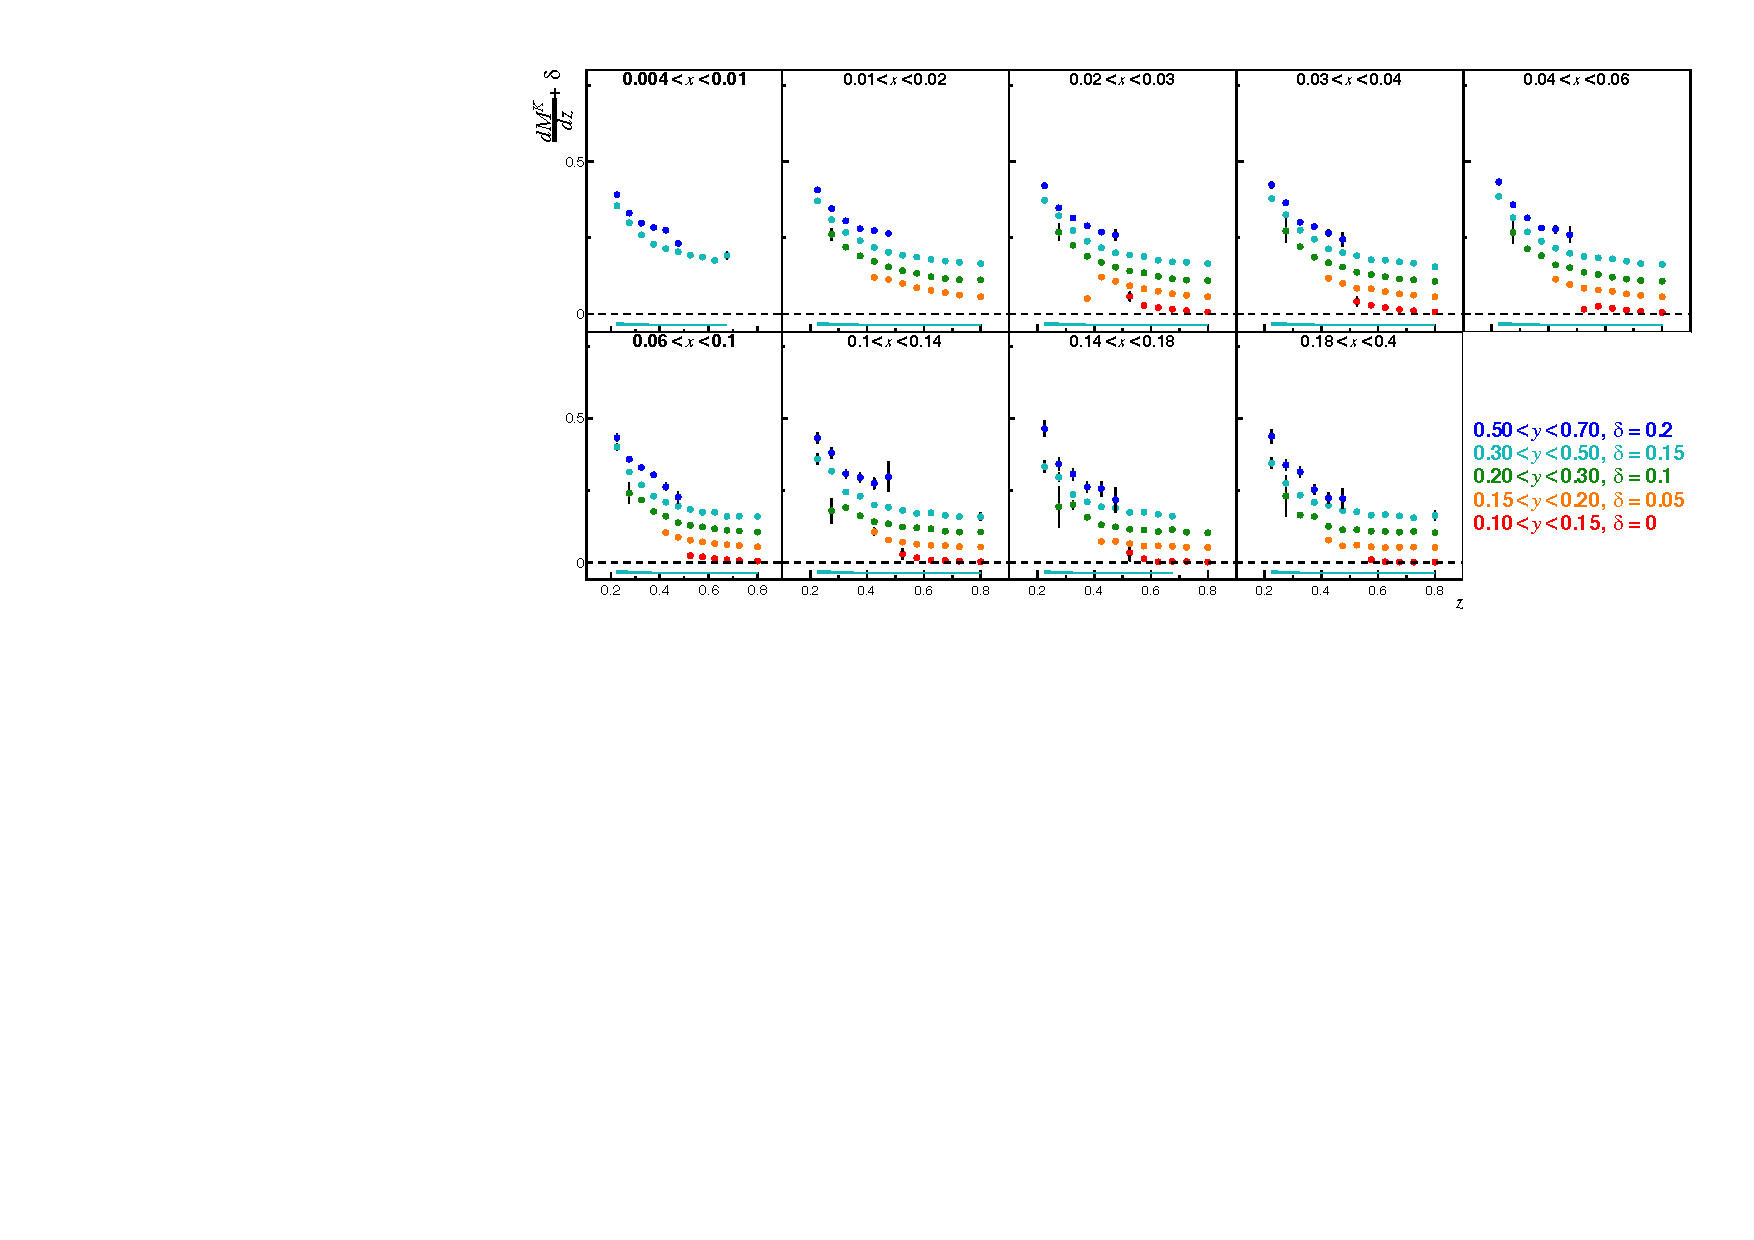
\includegraphics[scale=0.85]{./gfx/rawkm.pdf}
  \caption{Same as Fig.~\ref{pic:rawhp} but for negative pions.}
  \label{pic:rawkm}
\end{figure}

\begin{figure}[!h]
  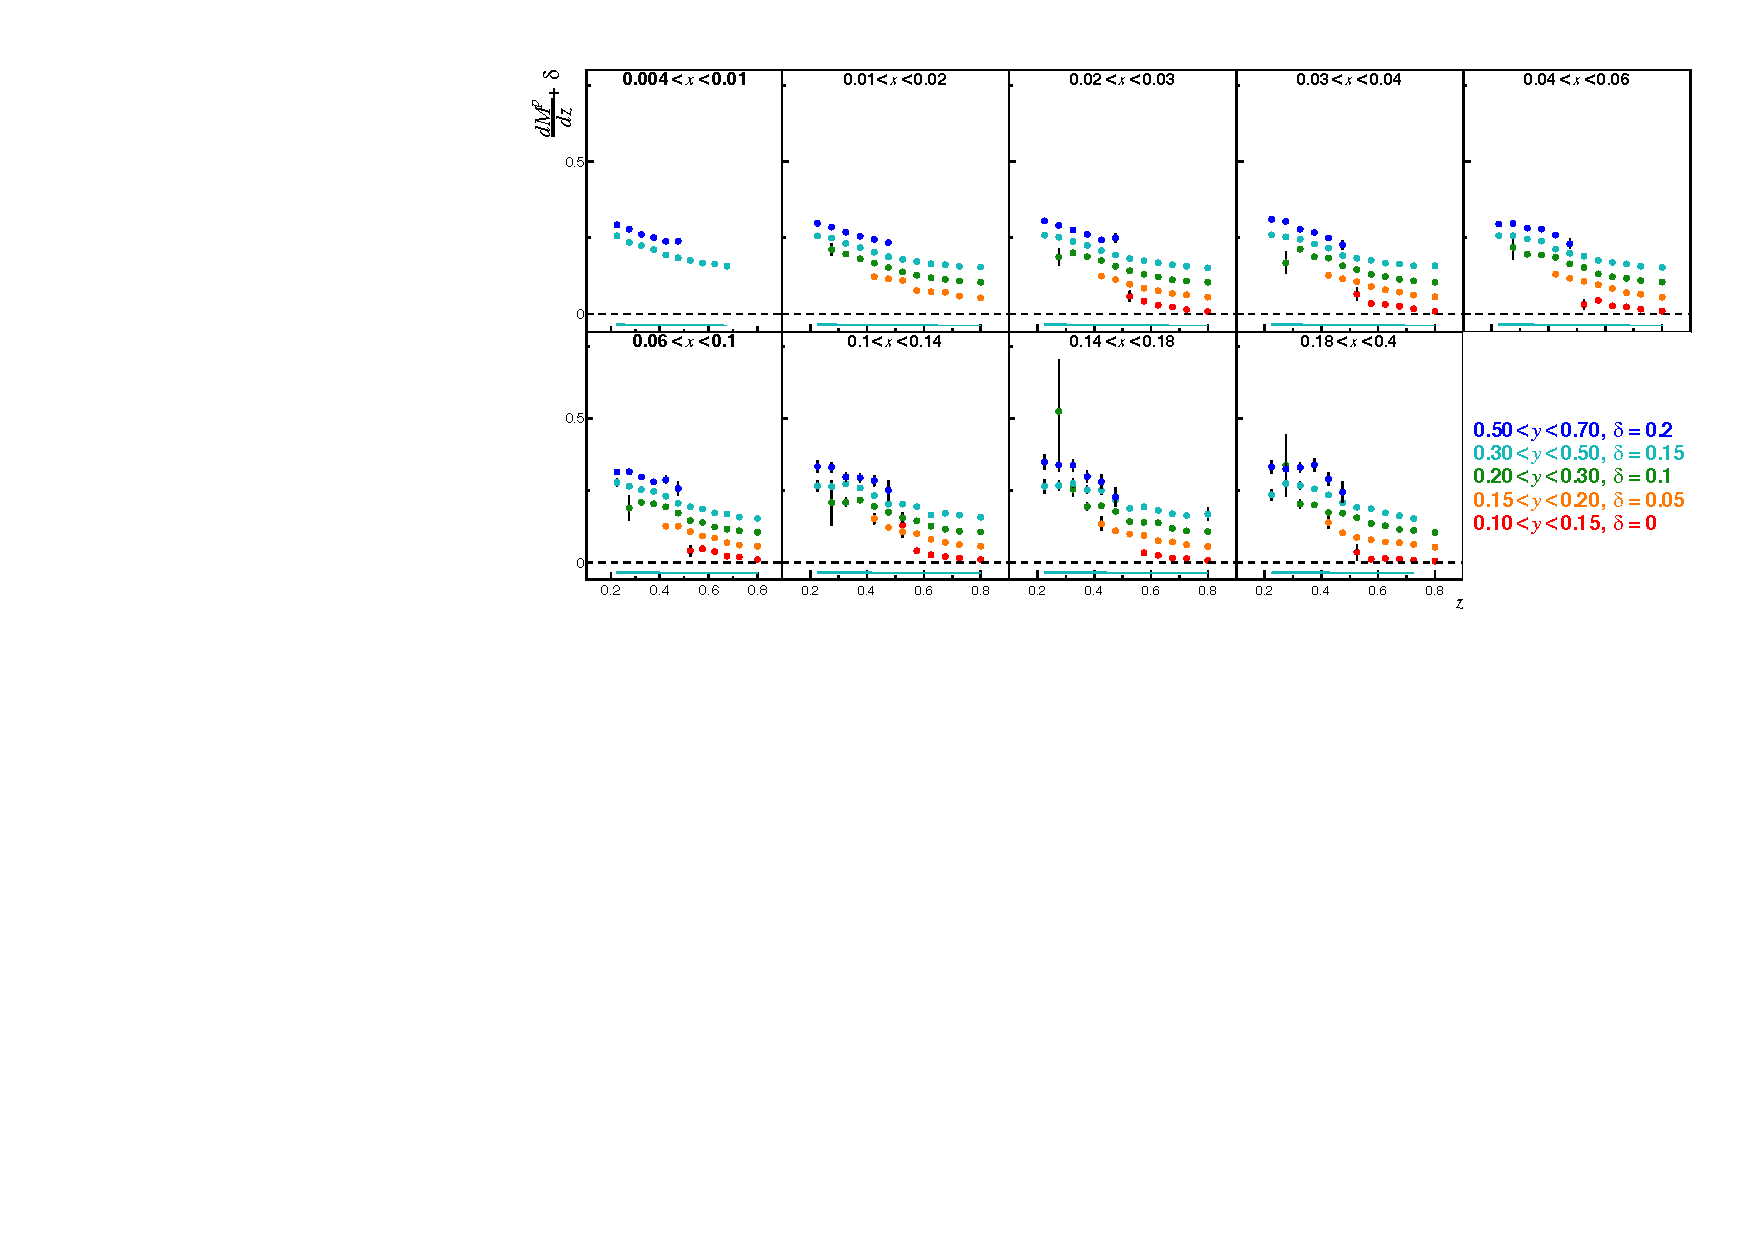
\includegraphics[scale=0.85]{./gfx/rawpp.pdf}
  \caption{Same as Fig.~\ref{pic:rawhp} but for protons.}
  \label{pic:rawpp}
\end{figure}

\newpage

\begin{figure}[!h]
  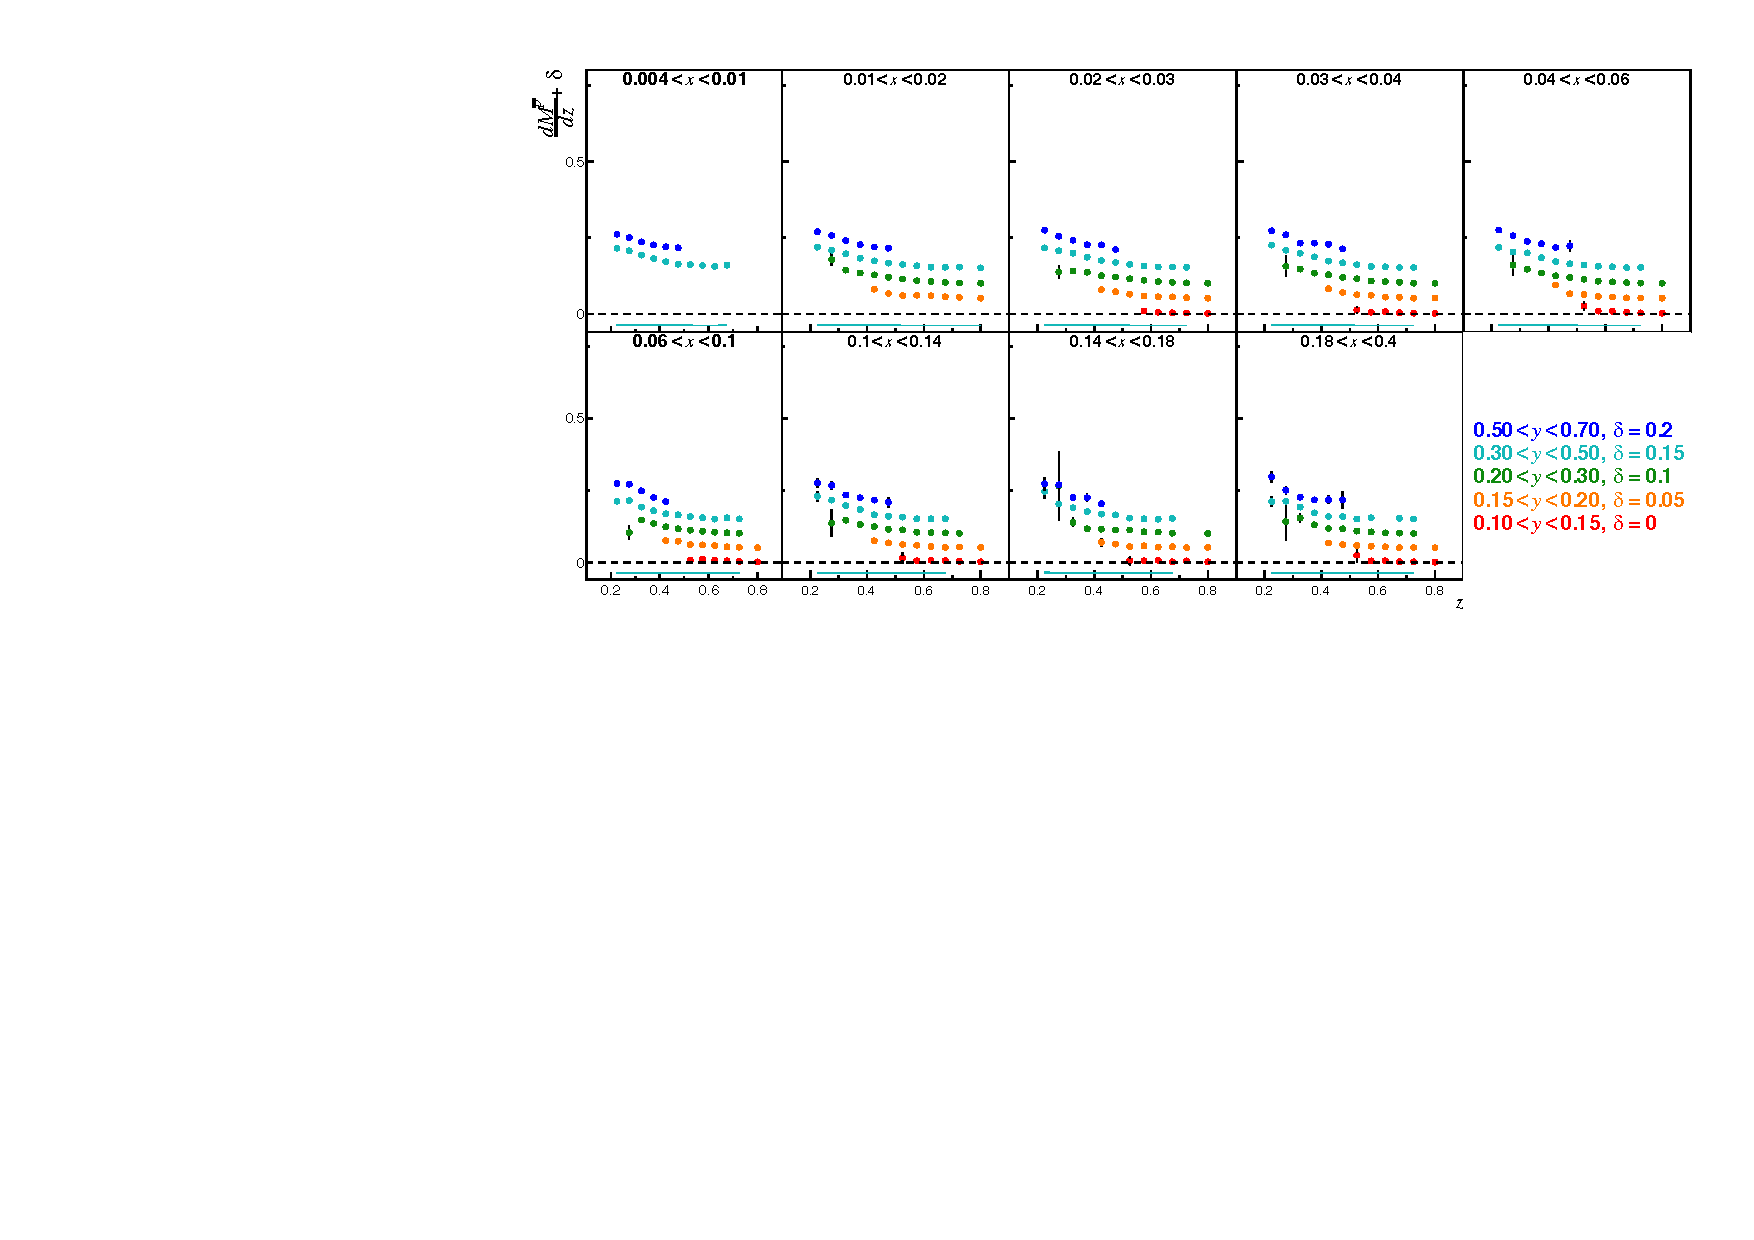
\includegraphics[scale=0.85]{./gfx/rawpm.pdf}
  \caption{Same as Fig.~\ref{pic:rawhp} but for antiprotons.}
  \label{pic:rawpm}
\end{figure}

\section{Summary}

From muon deep inelastic scattering on a pure proton target (lH$_2$) from the $2016$ COMPASS data, raw multiplicities for unidentified hadrons, pions, kaons and protons were extracted in a three dimensional ($x$,$y$,$z$) binning. The data cover a wide kinematic domain defined by $Q^2$ $>$ $1$ (GeV/$c$)$^2$, $y$ $\in$ [$0.1,0.7$], $x$ $\in$ [$0.004,0.4$], $W$ $\in$ [$5,17$] GeV and $z$ $\in$ [$0.2,0.85$]. The hadron momentum is taken in the range [$12,40$] GeV/$c$.

The raw multiplicities for identified hadrons are corrected by the RICH identification and misidentification efficiencies. The dominant uncertainty, before the application of correction factors, is the statistical error but for most of the bins $\sigma$/$M^h_{raw}$ < $1$\%.
